\chapter{Thiết kế định dạng văn bản riêng trong \LaTeX}\label{ch:3}
\section{Tổng quan về gói và lớp}\label{sec:3.1}
Như đã nói ở phần \hyperlink{package}{1.3}, người dùng hoàn toàn có thể tạo cho mình một lớp hoặc gói
nhằm bổ sung chức năng, môi trường mới cho văn bản, tự mình quy định bố cục, định dạng tuỳ theo mục
đích của văn bản mình muốn soạn thảo, hoặc chỉ đơn thuần tạo một quy chuẩn, mẫu có sẵn (form, template)
cho những văn bản trịnh trọng, học thuật hay báo cáo khoa học,\dots Các gói và lớp được tác giả chia sẻ cho cộng đồng (La)TeX,
sẽ được bảo hộ bằng giấy phép \acrshort{lppl}\footnote{\url{http://www.latex-project.org/lppl.txt}} và được 
lưu trữ trong \acrfull{ctan}, là tập hợp các trang web dùng để lưu trữ các gói, lớp của TeX
và LaTeX, được xây dựng vào năm 1992. \acrshort{ctan} có các bản lưu trữ dự phòng (mirror) chính thức ở một số
nước trên thế giới\footnote{\url{https://www.ctan.org/mirrors/}}, danh sách các nguồn tải ở hình \ref{fig:source} là một trong số đó. Do được
kết nối với các gói phân phối LaTeX, nên người dùng có thể tải các gói bổ sung trên \acrshort{ctan}
thông qua chúng, giúp tác giả của gói, lớp có thể dễ dàng phân phối, bảo trì và cập nhật sản phẩm của 
mình.\par
Người dùng có thể dễ dàng tạo gói và lớp bằng bất cứ trình soạn thảo nào và chỉ cần đặt tên
mở rộng của tập tin là \verb=.cls= (lớp) hoặc \verb=.sty= (gói), tuy nhiên, ta vẫn nên ưu tiên sử dụng trình soạn thảo
hỗ trợ LaTeX với lí do tương tự như khi soạn thảo thông thường (được highlight từ khoá và gợi ý câu lệnh). Việc tiếp theo là tuỳ theo
mục đích mà ta chọn tạo lớp hay gói. Thông thường, nếu muốn xây dựng, thiết kế bố cục, cấu trúc
logic của một loại văn bản tuỳ ý nào đó, ta sẽ tạo lớp, mặt khác, nếu  muốn xây dựng các câu lệnh,
môi trường và tính năng mới để sử dụng được trong bất kì loại văn bản nào, ta xây dựng gói.\par
\section{Giới thiệu lớp \texttt{vlththesis}}\label{sec:3.2}
Dựa vào giải thích trên và mục tiêu của đề tài này là thiết kế luận văn và bài báo cáo, nên sản phẩm
cuối cùng của đề tài sẽ là một tập tin lớp LaTeX (LaTeX class file), với các câu lệnh, canh chỉnh theo đúng quy định về
bố cục luận văn, bài báo cáo của trường và bộ môn. Lớp sản phẩm dựa trên lớp \texttt{book} của
LaTeX, mọi chi tiết về lớp \texttt{book} xin hãy tham khảo tài liệu thông tin các lớp tiêu chuẩn của LaTeX \cite{class}.
Ý tưởng một số câu lệnh trong đề tài này dựa trên lớp \texttt{gsemthesis}, là mẫu (template) đề tài tiến sĩ của trường đại học Geneva, Thuỵ Sĩ,
thông tin chi tiết về lớp này được nêu trong tài liệu hướng dẫn \cite{gsem}.\par
\section{Cấu trúc của \texttt{vlththesis}}\label{sec:3.3}
Phần này chủ yếu tập trung vào cấu trúc bên trong của \texttt{vlththesis} với các câu lệnh, khai báo, thông số
cũng như các gói kèm theo, cùng các thiết lập cho chúng.\par
\subsection{Các khai báo ban đầu}\label{subsec:3.3.1}
\lstinputlisting[firstline=1,lastline=4]{vlththesis.cls}

Câu lệnh \verb=\NeedsTeXFormat{LaTeX2e}[1999/12/01]=, trong đó \texttt{LaTeX2e} là bắt buộc \cite{latex-comp}, \path|[1999/12/01]|
là phiên bản tối thiểu của LaTeX 2$\varepsilon$ mà người viết tập tin yêu cầu máy người dùng đáp ứng,
hệ thống sẽ báo lỗi nếu người dùng sử dụng bản LaTeX cũ hơn phiên bản được nêu, do các gói phân phối
tự động tải về bản LaTeX mới nhất, người dùng không cần quá quan tâm đến thông số này.\par
Câu \verb=\ProvidesClass{vlththesis}= dùng để khai báo tên của lớp văn bản đang tạo và phải trùng với
tên của tập tin \texttt{.cls} được lưu, ở đây, tên khai báo là “\texttt{vlththesis}” và tên của file được
lưu là \path|vlththesis.cls|.\par
\lstinputlisting[firstline=5,lastline=5,firstnumber=last]{vlththesis.cls}

Là câu lệnh dùng để tải lớp, mà sản phẩm ta xây dựng, sẽ dựa trên, như đã nói ở \ref{sec:3.2}, lớp này dựa
trên \texttt{book} của LaTeX, kèm theo các tuỳ chọn đó là cỡ giấy A4 (\textbf{a4paper}), in và định dạng
một mặt giấy (\textbf{oneside}) và cỡ chữ \textbf{12pt} theo đúng chuẩn chung của một báo cáo khoá luận.\par
\lstinputlisting[firstline=7,lastline=8,firstnumber=7]{vlththesis.cls}

Lớp sử dụng gói \texttt{inputenc}, tuỳ chọn \textbf{utf8}, yêu cầu sử dụng bộ mã hoá (encoding) UTF-8 cho các kí tự trong văn
bản LaTeX như đã giải thích ở \ref{subsec:2.2.2}. \par \path|\RequirePackage{etoolbox}| dùng để nạp gói \texttt{etoolbox} chứa các
câu lệnh hỗ trợ viết các tập tin lớp, gói cho LaTeX \cite{etoolbox}.\par
\lstinputlisting[firstline=10,lastline=19,firstnumber=10]{vlththesis.cls}

Các câu lệnh \path|\DeclareOption{option name}{code}| trên dùng để khai báo các tuỳ chọn có trong lớp này mà người dùng có thể khai báo khi gọi lớp bằng câu lệnh \\ \path|\documentclass[option]{class}|,
trong đó, \textsl{code} là định nghĩa của tuỳ chọn, LaTeX sẽ tiến hành các câu lệnh trong phần này nếu người dùng khai báo tuỳ chọn \textsl{option name}.
Câu lệnh ở dòng 19 (\path|\ProcessOptions\relax|) là câu lệnh bắt buộc sau khi kết thúc việc khai báo và định nghĩa các tuỳ chọn có trong lớp, nó có chức
năng báo cho LaTeX phải xử lý các tuỳ chọn mà người dùng khai báo (nếu có) trước khi tiến hành các câu lệnh tiếp theo.\par 
Các tuỳ chọn mà \texttt{vlththesis} có được định nghĩa thông qua các câu lệnh trên như sau:\par
\lstinputlisting[firstline=10,lastline=11,firstnumber=10]{vlththesis.cls}
\clearpage 
Lớp cho phép sử dụng thêm tuỳ chọn \textbf{a5paper} của \texttt{book}, \path|\PassOptionsToClass{\CurrentOption}{book}| dùng
để báo cho LaTeX truyền tuỳ chọn đó vào \texttt{book} nếu người dùng khai báo nó, tuỳ chọn này sẽ được viết đè (override) tuỳ chọn mặc định \textbf{a4paper}
của lớp.\par 
Câu lệnh \path|\DeclareOption{twoside}{\OptionNotUsed}| dùng để ra cảnh báo nếu người dùng sử dụng tuỳ chọn in hai mặt \textbf{twoside}, do chuẩn bài báo
cáo chỉ yêu cầu in một mặt, người dùng có thể mở tập tin lớp này và thay đổi câu lệnh, sử dụng \path|\PassOptionsToClass{\CurrentOption}{book}|, nếu muốn sử dụng tuỳ chọn \textbf{twoside}. \par   
\lstinputlisting[firstline=12,lastline=13,firstnumber=last]{vlththesis.cls}

Lớp c định nghĩa tuỳ chọn mới: \hypertarget{viet}{\textbf{vietnamese}}, \path|\newtoggle| và \path|\toggletrue| là hai câu lệnh của \texttt{etoolbox},
\path|\newtoggle{viet}| định nghĩa một biến boolean mới tên “\texttt{viet}” và khi người dùng khai báo tuỳ chọn \textbf{vietnamese},
lớp sẽ thực hiện câu lệnh \\ \path|\toggletrue{viet}| trong phần định nghĩa và gán giá trị \texttt{true} cho biến \texttt{viet}.\par 
\lstinputlisting[firstline=14,lastline=17,firstnumber=last]{vlththesis.cls}

Các câu lệnh trên cũng thực hiện điều tương tự với dòng 12 và 13, đặt giá trị \texttt{true} cho các biến boolean mới
mỗi khi người dùng khai báo tuỳ chọn, chức năng hai tuỳ chọn này sẽ dần được nhắc đến ở các phần dưới.\par
\lstinputlisting[firstline=18,lastline=18,firstnumber=last]{vlththesis.cls}

Dùng để hiển thị cảnh báo nếu người dùng khai báo tuỳ chọn không được định nghĩa, bằng câu lệnh \path|\ClassWarning{vlththesis}{Unknown option '\CurrentOption'}|.
\path|\DeclareOption*{code}|, khác với \path|\DeclareOption|, chỉ nhận đầu vào \textsl{code} và dùng để xử lý bất kì tuỳ chọn nào, do đó
nó thường được dùng để xử lý các tuỳ chọn không được định nghĩa hoặc dùng chung với câu \path|\PassOptionsToClass{\CurrentOption}{class}| để
kế thừa toàn bộ các option của lớp mà sản phẩm hiện hành dựa trên. LaTeX sẽ tiến hành tìm kiếm định nghĩa của tuỳ chọn được khai báo
trước khi đẩy tuỳ chọn vào \path|\DeclareOption*{code}|, nếu không tìm thấy định nghĩa của tuỳ chọn cũng như \path|\DeclareOption*|, LaTeX
vẫn tiếp tục chạy tập tin đầu vào nhưng sẽ hiển thị cảnh báo.\par 
 
\subsection{Khai báo gói và thiết lập}\label{sec:3.3.2}
Dưới đây là các đoạn lệnh dùng để khai báo và thiết lập thông số cho các gói được sử dụng trong lớp này. Khai báo
lớp đồng nghĩa với việc người dùng đã khai báo các gói tích hợp, người dùng hoàn toàn có thể thay đổi các thiết lập
sau tuỳ thích sử dụng câu lệnh tương tự, khi soạn thảo tập tin đầu vào.\par 
\lstinputlisting[firstline=21,lastline=27,firstnumber=21]{vlththesis.cls}

Câu lệnh điều kiện \path|\iftoggle{boolean}{true condition}{false condition}| của \texttt{etoolbox},
sẽ tiến hành kiểm tra biến trong \textsl{boolean}, nếu biến mang giá trị \texttt{true}, câu lệnh trong phần
\textsl{true condition} được thực h, và ngược lại, lệnh ở phần \textsl{false condition} sẽ được triển khai nếu biến là \texttt{false}.
Như đã nói ở \hyperlink{viet}{3.3.1}, \texttt{viet} mang giá trị \texttt{true} khi người dùng khai báo tuỳ chọn \textbf{vietnamese}, 
khi đó, câu lệnh thực hiện phần \textsl{true condition}, tức ba câu lệnh từ dòng 22 tới 24.\par
Ba câu lệnh ở điều kiện \texttt{true}, dùng để nạp gói \texttt{babel} tuỳ chọn \textbf{vietnamese} để hỗ trợ xử lý tiếng Việt, người dùng phải tải thêm ngôn ngữ tiếng Việt cho \texttt{babel}
bằng cách sử dụng \texttt{yum} hoặc \texttt{apt-get} kèm theo \texttt{install texlive-babel-vietnamese}.
Gói \texttt{hyphsubst}, dùng để ngăn LaTeX đưa cảnh báo về ngắt chữ khi xuống dòng (tập tin đầu vào vẫn được chạy bình thường khi
có cảnh báo này, việc sử dụng gói \texttt{hyphsubst} chỉ đơn thuần nhằm hạn chế các cảnh báo không cần thiết). Gói \texttt{indentfirst}
cho phép LaTeX thụt đầu dòng đoạn văn (paragraph) đầu tiên của một chương, đề mục,\dots \par
Khi biến \texttt{viet} có giá trị \texttt{false} (tức người dùng không khai báo tuỳ chọn \textbf{vietnamese}), câu lệnh ở phần \textsl{false condition}
sẽ được thực hiện, đó là nạp package \texttt{babel} với tuỳ chọn \textbf{english} để hỗ trợ trình bày tiếng Anh.\par
Phần khai báo tiếp theo sẽ là về các gói phụ trợ không kèm theo các thiết lập thông số đặc biệt:\par
\clearpage 
\lstinputlisting[firstline=28,lastline=39,firstnumber=last]{vlththesis.cls}

Package \texttt{geometry} dùng để canh chỉnh lề cho trang giấy và là một trong những gói cơ bản của LaTeX, có sẵn khi tải distribution,
option của package này thường là các thông số, kích thước cho lề của mặt giấy. Class sử dụng package để khai báo canh lề cho trang giấy
với các thông số: left (lề trái) 1.38 inch, right (lề phải) 0.79 inch, top (lề đầu bao gồm header) 1.15 inch và bottom (lề cuối bao gồm
footer) 1.15 inch.\par
Package \texttt{graphicx} như đã nhắc tới ở phần \hyperlink{graphicx}{2.2.2}, dùng để thêm hình ảnh vào văn bản và là một trong những 
package cơ bản, có sẵn.
Package \texttt{multirow} cho phép tạo bảng gôm (merge) nhiều cột, dòng sử dụng trong môi trường \textbf{\slshape tabular} ở phần \hyperlink{table}{2.2.2},
chi tiết về cách gôm nhiều cột dòng người dùng có thể xem hướng dẫn, ví dụ ở ShareLateX \cite{sharelatex} hoặc tài liệu của package này \cite{multirow}.\par
Package \texttt{wrapfig} cung cấp thêm môi trường \textbf{\slshape wrapfigure} và \textbf{\slshape wraptable} dùng để tạo hiệu ứng chữ
bao lấy hình ảnh và bảng (giống với hiệu ứng Square của trình soạn thảo Microsoft Word), cách sử dụng môi trường này được cung cấp trong tài liệu
\cite{wrapfig} và các ví dụ sử dụng cũng được tìm thấy ở trang \cite{sharelatex}.\par
Package \texttt{array} cung cấp thêm giá trị canh chỉnh mới cho \textbf{\slshape tabular} ngoài \texttt{\bfseries l}, \texttt{\bfseries r} và \texttt{\bfseries c} (xem phần \hyperlink{table}{2.2.2}, phần hướng dẫn thêm hình
và bảng để biết thêm chi tiết) đó là \texttt{\bfseries m{width}} và \texttt{\bfseries b{width}}, cho phép ta nhập đoạn văn dài vào bảng đồng thời xác định
chiều rộng ô với \textsl{width}, chi tiết về package này và môi trường \textbf{\slshape tabular} sẽ được tìm thấy trong tài liệu hướng dẫn \cite{array}.\par 
Package \texttt{float} cung cấp một biến thể của giá trị \textsl{placement} \texttt{\bfseries h}, của môi trường \textbf{\slshape figure}, đó là \texttt{\bfseries H}.
Biến thể này chặt chẻ hơn \texttt{\bfseries h}, và dùng trong trường hợp \texttt{\bfseries h} không đặt hình ở vị trí mình mong muốn.\par
Các package \texttt{amsmath,amsfonts,amssymb} cung cấp font chữ, câu lệnh, định dạng, canh chỉnh cho các công thức và kí hiệu toán học, cũng như
văn bản cho các môi trường dùng để soạn thảo công thức (như \textbf{\slshape equation} hay \textbf{\slshape align}), các package này được chính
\acrshort{ams} phát triển.\par  
Package \texttt{tocbibind} dùng để hiển thị “Danh sách hình ảnh” và “Danh sách bảng” lên mục lục, mặc định LaTeX sẽ không để các phụ
chương không được “đánh số” (unnumbered) lên mục lục, \texttt{notoccite} dùng để hạn chế một số trường hợp các câu lệnh dẫn nguồn (\verb=\cite=)
bị liệt kê trên mục lục \cite{notoccite}, package \texttt{path} cung cấp câu lệnh \verb=\path| |=, cho ta đánh dấu đường dẫn, câu lệnh, email,\dots
trong văn bản LaTeX, nội dung bên trong sẽ được định dạng bằng font chữ \texttt{monospace} và các kí tự đặc biệt trong đó sẽ được xem như kí tự bình thường
(giống như khi ta “comment” trong một file code). Package \texttt{totalcount} dùng để kiểm tra và đếm số lượng bảng, hình trong văn bản, người dùng bình thường
không cần phải quá quan tâm đến gói này.\par
\textsl{\bfseries Lưu ý}: Các package \texttt{multirow, wrapfig, tocbibind, notoccite, path} có thể không có sẵn trong distribution,
người dùng cần phải tải bổ sung nếu hệ thống báo thiếu, cách tải package LaTeX bổ sung trong Linux được nêu ở phần \ref{subsec:2.1.1}.\par 
Tiếp theo là các package kèm theo các thiết lập thông số: \par
\lstinputlisting[firstline=40,lastline=41,firstnumber=40]{vlththesis.cls}

Tương tự như gói \texttt{path}, package \texttt{url} cung cấp câu lệnh \verb=\url| |= để ta đánh dấu địa chỉ URL của website, option
\textbf{obeyspaces} cho phép hiển thị khoảng cách (nếu có) trong địa chỉ (điều hiếm khi xảy ra), package còn cung cấp câu lệnh 
\verb=\urlstyle= cho phép ta đề ra các thiết lập định dạng cho URL như font, cỡ chữ,\dots. Ở đây, các URL được đánh dấu bằng
\verb=\url| |= sẽ có font chữ Sans Serif (sf). Người dùng có thể thay đổi thiết lập này, sử dụng câu lệnh tương tự, các thay đổi
có thể được thực hiện bằng câu lệnh này được liệt kê trong tài liệu \cite{url} của package.\par 
\lstinputlisting[firstline=43,lastline=43,firstnumber=43]{vlththesis.cls}

Tiếp theo là package \texttt{titlesec} dùng để định dạng đề mục, đây là package có sẵn trong distribution, class này sử dụng hai câu 
lệnh chính của \texttt{titlesec} là \path|\titleformat| và \path|\titlespacing*|, lưu ý rằng \path|\titlespacing*| chỉ có thể sử dụng
được khi có \\ \path|\titleformat| trước nó \cite{titlesec}. Ta xét cú pháp hai câu lệnh đó:\par
\clearpage 
\begin{center}
 \path|\titleformat{command}[shape]{format}{label}{sep}{before-code}[after-code]|
\end{center}

Trong đó:\par
\begin{itemize}
 \item <command> là câu lệnh đề mục mà ta muốn thay đổi, như \path|\part|, \path|\chapter|, \path|\section|,\dots
 \item <shape> là kiểu bố trí thành phần đề mục như hang, block, display,\dots chi tiết về các kiểu bố trí được nêu trong \cite{titlesec}.
 \item <format> dùng để định dạng font, cỡ chữ, canh chỉnh cho nhãn và tiêu đề chương.
 \item <label> dùng để quy định cách trình bày nhãn của đề mục ví dụ “Chương 2” thành “Chương II.”.
 \item <sep> là khoảng cách giữa nhãn và tiêu đề của đề mục.
 \item <before-code> và <after-code> dùng để bổ sung những câu lệnh ta muốn LaTeX thực hiện trước và sau
 khi trình bày tiêu đề.
\end{itemize}

\begin{center}
 \path|\titlespacing*{command}{left}{before-sep}{after-sep}[right-sep]|
\end{center}

Trong đó:\par
\begin{itemize}
 \item <command> tương tự như với \path|\titleformat|.
 \item <left> khoảng cách giữa lề trái và tiêu đề.
 \item <before-sep> là khoảng cách từ lề đầu của trang đến tiều đề.
 \item <after-sep> là khoảng cách giữa tiêu đề và nội dung văn bản.
 \item <right-sep> khoảng cách giữa lề phải và tiêu đề.
\end{itemize}

Hai câu lệnh trên được sử dụng trong class này nhằm thay đổi bố cục mặc định của tiêu đề trước tiên
là các đề mục phụ (không chia số chương như “Lời giới thiệu”, “Lời cảm ơn”,\dots) còn gọi là unnumbered hay numberless chapter.\par
\lstinputlisting[firstline=44,lastline=47,firstnumber=last]{vlththesis.cls}

Câu \verb=\titleformat= trên sử dụng thông số định dạng tương tự với định dạng mặc định của LaTeX
dành cho đề mục không đánh số, chỉ có một số thay đổi đó là câu lệnh \path|\filcenter| để canh giữa
và cỡ chữ từ \verb=\Huge= sang \verb|\LARGE|, nhỏ hơn hai bậc so với \verb|\Huge|, để thu nhỏ tiêu đề
so với định dạng mặc định. Do \verb|\titlespacing*| cần phải đi kèm với \verb=\titleformat= trước, nên
giả sử nếu ta chỉ muốn thay đổi khoảng cách tiêu đề, ta cũng phải sử dụng \verb=\titleformat= với các
định dạng mô phỏng lại giống hoặc gần giống với định dạng mặc định, với \verb|\titlespacing*|, class
cũng thay đổi khoảng cách từ lề đầu đến tiêu đề, số âm ở giá trị cho thấy, đề mục lấn ra phần header, tuy
nhiên, do tiêu đề ở trang đầu của một chương được coi là header, nên class tạm thời “mượn” khoảng đó để đặt đề mục.
Kết quả có được khi đặt hai câu lệnh đó và sử dụng class này thay cho class \texttt{book} thông thường như sau:\par
\begin{figure}[H] 
 \begin{subfigure}{0.5\textwidth}
  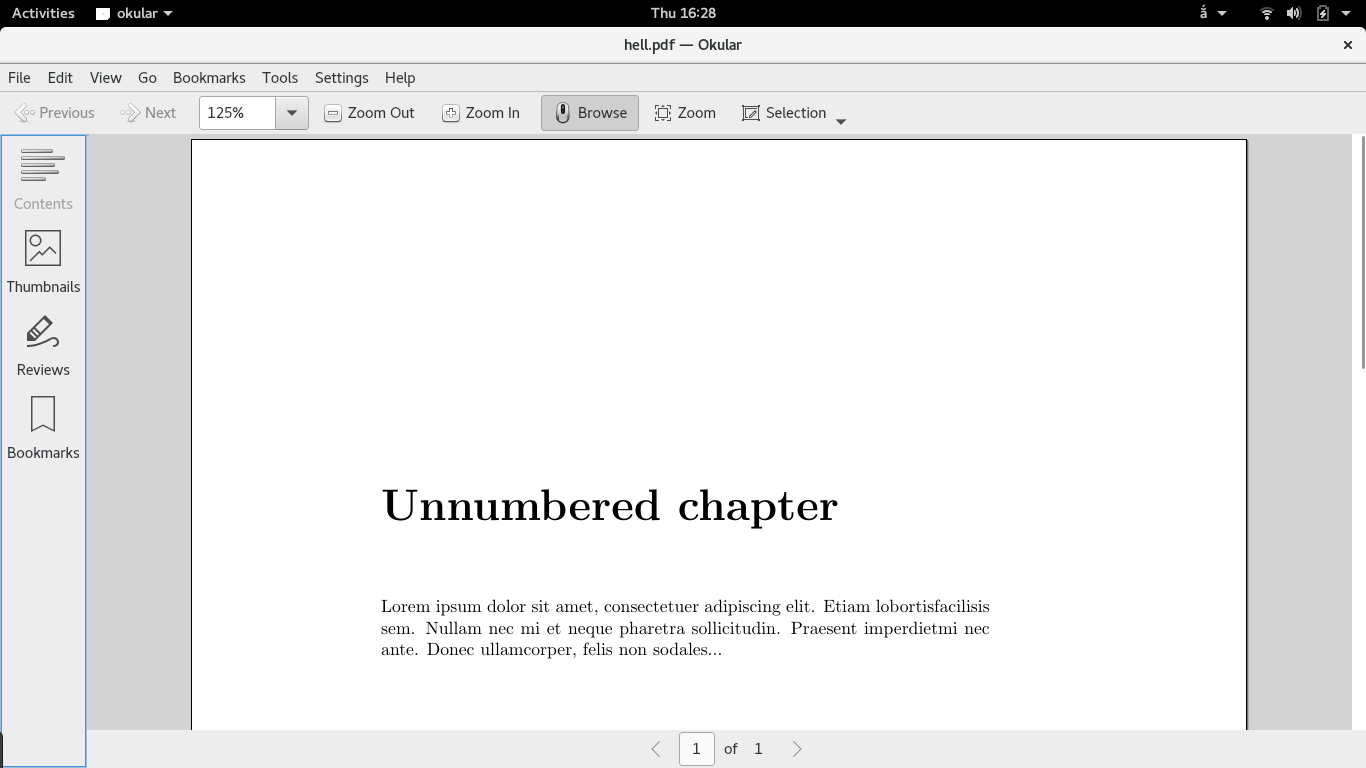
\includegraphics[width=1.\linewidth]{titlesec_a}
  \caption{Sử dụng class \texttt{book}}
  \label{fig:titlesec_a}
 \end{subfigure}
 \begin{subfigure}{0.5\textwidth}
  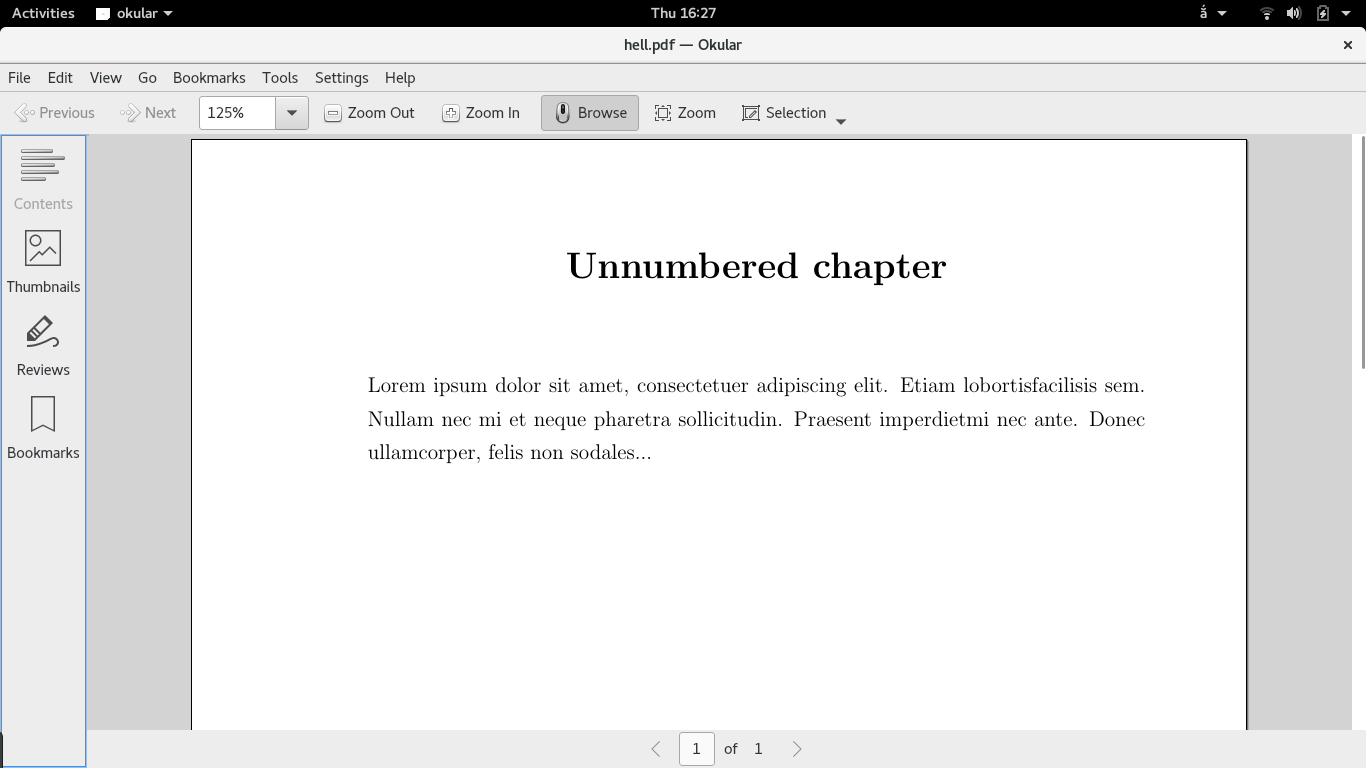
\includegraphics[width=1.\linewidth]{titlesec_b}
  \caption{Sử dụng class \texttt{vlththesis}}
  \label{fig:titlesec_b}
 \end{subfigure}

 \caption{So sánh đề mục của hai class văn bản}
 \label{fig:titlesec}
\end{figure}

Tiếp theo là câu lệnh dành cho đề mục chương có đánh số (numbered chapter):\par
\lstinputlisting[firstline=49,lastline=61,firstnumber=49]{vlththesis.cls}

Đề mục chương đánh số cũng có thông số \verb|\titlespacing*| gần giống với không đánh số, sự khác nhau là do chương đánh số có
kèm theo nhãn (chữ “Chương\dots” hay “Chapter\dots”), phần \verb=\titleformat= dùng để canh giữa và bổ sung thêm các đường kẻ (ruler)
và thay đổi cỡ chữa nhỏ hơn so với mặc định. Kết quả có được là:\par
\begin{figure}[H] 
 \begin{subfigure}{0.5\textwidth}
  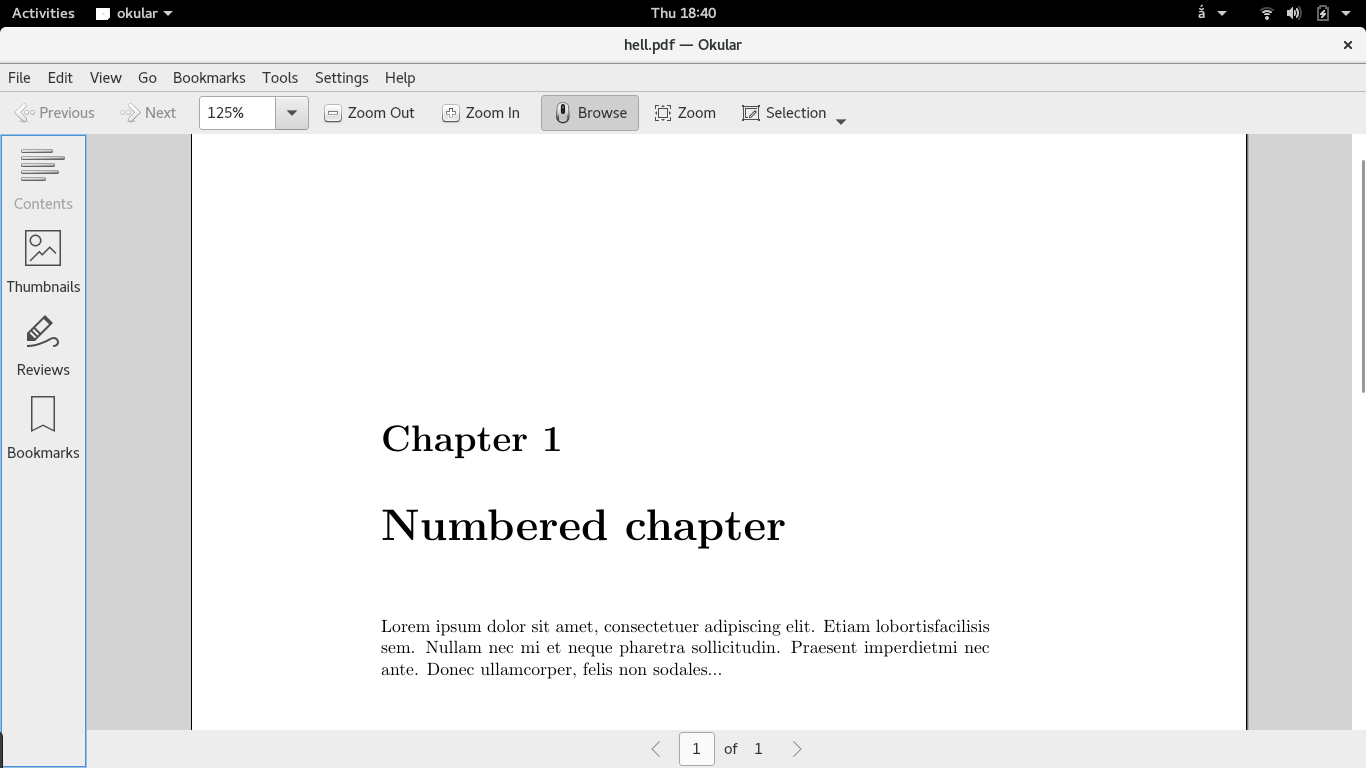
\includegraphics[width=1.\linewidth]{titlesec2_a}
  \caption{Sử dụng class \texttt{book}}
  \label{fig:titlesec2_a}
 \end{subfigure}
 \begin{subfigure}{0.5\textwidth}
  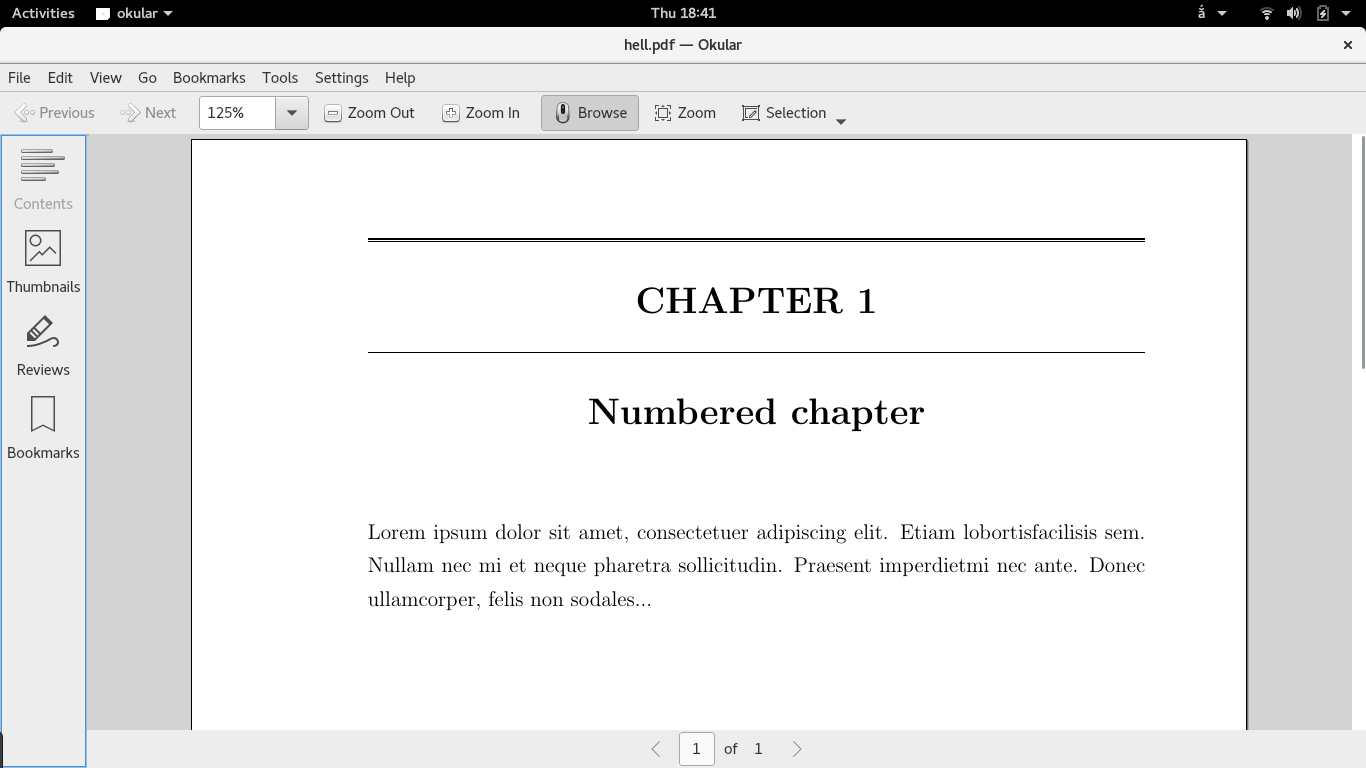
\includegraphics[width=1.\linewidth]{titlesec2_b}
  \caption{Sử dụng class \texttt{vlththesis}}
  \label{fig:titlesec2_b}
 \end{subfigure}

 \caption{So sánh đề mục (có đánh số) của hai class văn bản}
 \label{fig:titlesec2}
\end{figure}

Tiếp theo là package \texttt{caption} và \texttt{subcaption}:\par
\lstinputlisting[firstline=63,lastline=70,firstnumber=63]{vlththesis.cls}

Trong đó package \texttt{caption} cho phép ta định dạng chú thích cho bảng và hình (caption) thông qua câu lệnh \path|\captionsetup|
bằng cách sử dụng khai báo kiểu key-value như trên từ font chữ (\textsl{font}, \textsl{labelfont}, \textsl{textfont}), định dạng (\textsl{format}), 
và độ rộng cho phép (\textsl{width}),\dots Để biết thêm các giá trị key cũng như value tương ứng mà ta có thể dùng để định dạng caption, 
người dùng có thể tham khảo thêm trong tài liệu \cite{caption}.\par Package \texttt{subcaption} là gói đi kèm với \texttt{caption} và cả hai
đều có sẵn trong distribution, \texttt{subcaption} cho phép ta chèn nhiều hình phụ với một caption chung, ví dụ cho dạng trình bày này chính là
các hình \ref{fig:kile}, \ref{fig:titlesec} và \ref{fig:titlesec2} ở trên,
bên cạnh đó package cho phép các hình phụ có caption riêng với môi trường \textbf{\slshape subfigure} do nó cung cấp, 
ngoài ra package còn bổ sung thêm option \texttt{sub}
cho câu lệnh \verb|\captionsetup| (\verb|\captionsetup[sub]|) cho phép caption phụ có định dạng riêng.\par
Nhờ tích hợp câu lệnh trên mà class này có định dạng caption khác với \texttt{book}.\par
\begin{figure}[H] 
 \begin{subfigure}{0.5\textwidth}
  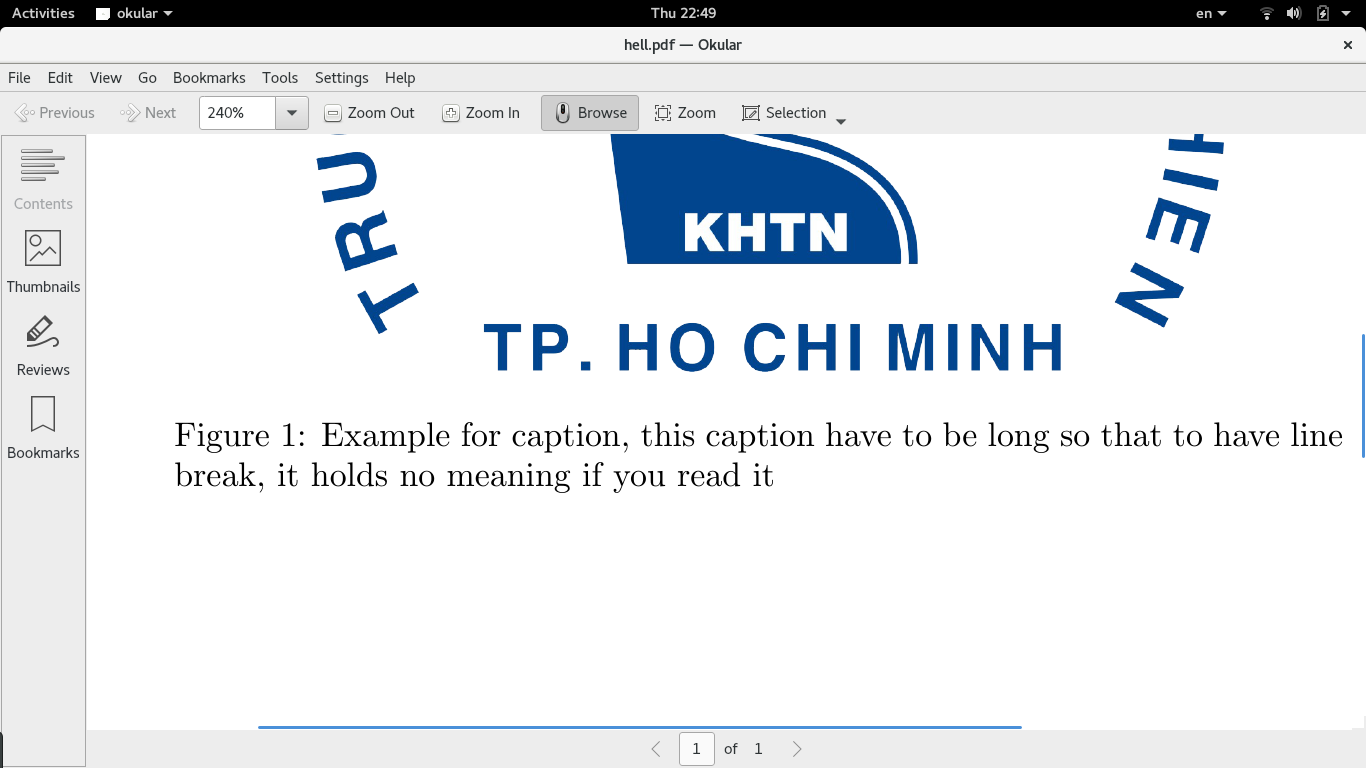
\includegraphics[width=1.\linewidth]{caption_a}
  \caption{Sử dụng class \texttt{book}}
  \label{fig:caption_a}
 \end{subfigure}
 \begin{subfigure}{0.5\textwidth}
  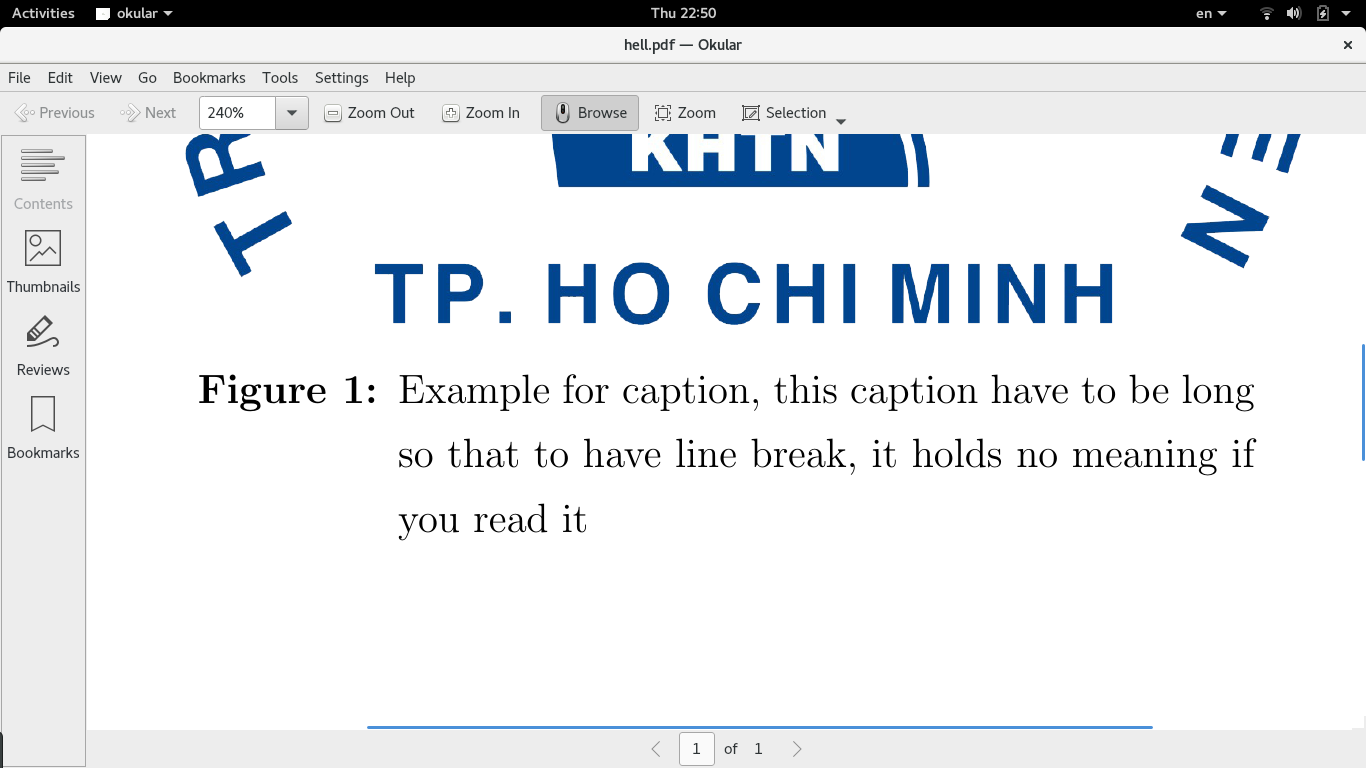
\includegraphics[width=1.\linewidth]{caption_b}
  \caption{Sử dụng class \texttt{vlththesis}}
  \label{fig:caption_b}
 \end{subfigure}

 \caption{So sánh caption của hai class văn bản}
 \label{fig:caption}
\end{figure}

Các dòng tiếp theo là khai báo và sử dụng package \texttt{xcolor}:\par
\lstinputlisting[firstline=72,lastline=78,firstnumber=72]{vlththesis.cls}

Ở đây tôi sử dụng câu lệnh \verb|\definecolor| để định nghĩa một số màu sắc sẽ sử dụng trong class này. Package \texttt{xcolor} cho 
phép ta tạo màu sử dụng các mã màu thông dụng như HTML, RGB,\dots và cung cấp câu lệnh cho phép ta 
định màu cho một câu chữ hay đoạn văn bản, nếu người dùng quan tâm muốn biết thêm các chức năng
câu lệnh có trong package có thể tham khảo trong \cite{xcolor} hoặc trang web hướng dẫn ShareLaTeX \cite{sharelatex}.\par
Tiếp đến là các khai báo cho package \texttt{hyperref}.\par

\lstinputlisting[firstline=80,lastline=88,firstnumber=80]{vlththesis.cls}
\clearpage
\lstinputlisting[firstline=89,lastline=91,firstnumber=last]{vlththesis.cls}

Package \texttt{hyperref}, dùng để tạo, thiết lập thuộc tính cho các siêu liên kết (hyperlink) trong văn bản (liên kết nội, url,\dots), và là
một package cơ bản có sẵn, option \path|linktocpage=true| để
biến số trang trên mục lục thành liên kết dẫn đến trang đó (thay vì mặc định là cả tiêu đề trong mục lục là liên kết).\par
Tương tự như \texttt{caption}, \texttt{hyperref} cung cấp câu lệnh \path|\hypersetup| cho ta định màu sắc cho từng loại liên kết, tinh
chỉnh hành vi, định dạng của chúng bằng key-value. Trong class này, tôi sử dụng những màu sắc đã tạo bằng \path|\definecolor| cho
các loại liên kết khác nhau như liên kết nội bộ (\texttt{linkcolor}), liên kết file bên ngoài (\texttt{filecolor}), liên kết url (\texttt{urlcolor})
và liên kết dẫn nguồn (\texttt{citecolor}). \path|colorlinks=true| dùng để bật tính năng màu cho liên kết và phải \texttt{true} nếu người dùng
muốn định màu cho các liên kết và \path|breaklinks=true| cho phép liên kết được xuống hàng như văn bản bình thường.\par 
Câu \path|\iftoggle{print}| để kiểm tra người dùng có khai báo option \textbf{print} của class
hay không, nếu biến boolean \texttt{print} là \texttt{true} (người dùng có khai báo) tiến hành tắt tính năng tô màu cho liên kết (\path|colorlinks=false|), tuy nhiên, các
liên kết đó vẫn được đánh dấu bằng các ô vuông theo màu mặc định của LaTeX (không phải màu do người dùng định), mục đích của tính năng này là do khi in
văn bản ra, các màu link vẫn được giữ nguyên trên bản in nếu người dung in màu, vì vậy cần phải bổ sung thêm option này để tắt màu liên kết.\par
\lstinputlisting[firstline=93,lastline=99,firstnumber=93]{vlththesis.cls}

Package \texttt{fancyhdr} dùng để tạo và định dạng header và footer, với các câu lệnh \path|\fancyhead| và \path|\fancyfoot|, người dùng
có thể quy định vị trí và nội dung hiển thị trên header và footer (như số trang, tên chương,\dots). Với package này, người dùng có thể đặt
bố cục cho một trang nhất định hay cả văn bản (sử dụng \path|\pagestyle| hoặc \path|\thispagestyle|), định dạng, đặt tên bố cục header, footer cho
riêng mình (\path|\fancypagestyle|). Các kiểu bố cục (style) có sẵn thường được dùng là: \texttt{empty} (không header hay footer), \texttt{plain} (chỉ có số trang ở giữa footer)
và \texttt{fancy} (do người dùng định ra sử dụng \path|\fancyhead| và \path|\fancyfoot|), ngoài ra còn có \texttt{myheadings}, chi tiết về các mẫu 
bố cục và các thao tác với package này có thể được tìm thấy trong tài liệu \cite{fancyhdr}.\par

Ở đoạn code trên, ta có \path|\pagestyle{fancy}| dùng để đặt style \texttt{fancy} cho cả văn bản, kế
đến là phần thiết kế bố cục, trong đó, \path|\fancyhf{}| để xoá các header, footer 
hiện hành, đây chỉ là buớc reset trước khi định dạng, câu lệnh \path|\fancyhead[R]| dùng để đặt 
\path|\rightmark| (tức tiêu đề và nhãn mục của đơn vị chương hồi \emph{thấp nhất} của trang nội dung hiện t, xem bảng \ref{tab:chapter}
để biết thêm về thứ bậc chương) vào ví trí bên phải của header (\texttt{R} ứng với vị trí phải).
Câu lệnh \path|\fancyhead[L]| để đặt \path|\chaptertitlename\ \thechapter| vào vị trí bên trái (\texttt{L=Left}),
trong đó, \path|\chpatertitle| chính là “Chương” hay “Chapter” (tuỳ theo ngôn ngữ hiện hành của \texttt{babel} mà
chữ này có thể khác nhau) và \path|\thechapter| chính là số chương hiện hành của trang. Tiếp theo, 
\path|\fancyfoot[C]| dùng để đặt \path|\thepage|, tức số trang ở phần giữa (\texttt{C=Center}) cho footer,
cuối cùng là \path|\renewcommand{\headrulewidth}| để tạo đường kẻ cho header.\par
\textbf{\slshape Lưu ý}: Nếu không nêu rõ các thiết lập trên là của style gì (bằng cách sử dụng câu lệnh \path|\fancypagestyle{tên style}{các thiết lập}|)
package sẽ mặc định hiểu đó là của style \texttt{fancy}.\par 
Sau khi tiến hành thực hiện các câu lệnh trên, kết quả có được chính là bố cục header và footer của cuốn
báo cáo này. Ngoài bố cục này, class còn có thêm \hypertarget{appendix}{bố cục khác} dùng cho phụ lục:\par
\lstinputlisting[firstline=101,lastline=106,firstnumber=101]{vlththesis.cls}

Tiếp theo là package hỗ trợ nhập code vào văn bản LaTeX.\par
\lstinputlisting[firstline=109,lastline=109,firstnumber=109]{vlththesis.cls}

Đây là package cung cấp các câu lệnh dùng để định dạng từ khoá và hỗ trợ in code cho văn bản LaTeX, vốn
được cộng đồng xem là một bảng nâng cấp của môi trường \textbf{\slshape verbtim} và câu lệnh \path|\verb|
của LaTeX. Câu lệnh cung cấp môi trường \textbf{\slshape lstlisting} với các option dạng key-value cho phép
in số dòng cho code theo nhiều cách tuỳ thích, nhận dạng câu lệnh, từ khoá của ngôn ngữ lập trình (danh sách
các ngôn ngữ được hỗ trợ có trong \cite{lstlisting}) từ đó cho người dùng định màu sắc cho các loại từ khoá đó
như trường hợp các loại liên kết trong \texttt{hyperref}, người dùng thậm chí còn có thể định danh ngôn ngữ không được hỗ
trợ sẵn trong package, như trường hợp sau đây là một đoạn code có trong class dùng để định nghĩa ngôn
ngữ JavaScript do cộng đồng LaTeX chia sẻ:\par
\lstinputlisting[firstline=111,lastline=120,firstnumber=111]{vlththesis.cls}

Ta có thể thấy ngôn ngữ được định nghĩa bằng các giá trị key-value trong câu lệnh \path|\lstdefinelanguage|, ý nghĩa của
các giá trị này bao gồm liệt kê từ khoá của ngôn ng (\texttt{keywords, ndkeywords}), ngôn
ngữ có phân biệt chữ hoa và thường hay không (\texttt{sensitive}), định ra kí hiệu ghi chú
(comment) của ngôn ngữ (\texttt{comment, morecomment}) và kí hiệu chuỗi (\texttt{morestring}).\par
Cũng như các \texttt{caption, hyperref},\dots package cũng có \path|\lstset| giúp ta
chỉnh sửa định dạng cho môi trường \textbf{\slshape lstlisting}, các định dạng sử dụng trong class
này như sau:\par 
\lstinputlisting[firstline=123,lastline=140,firstnumber=123]{vlththesis.cls}

Các định dạng bao gồm kiểu, cỡ chữ hay màu sắc chung cho toàn bộ đoạn code (\texttt{basicstyle}), cho các từ khoá của ngôn ngữ lập trình
(\texttt{keywordstyle}), cho các ghi chú (\texttt{commentstyle}) và chuỗi (\texttt{basicstyle}), tuỳ chỉnh vị trí hoặc bật tắt đánh
số dòng (\texttt{numbers}),\dots Một số giá trị key để trống nhầm gợi ý tính năng cho những ai có mong muốn tinh chỉnh định dạng của
\texttt{lstlisting}, tất nhiên các định dạng này có thể được ghi đè (override) hoặc bổ sung bởi \path|\lstset| của người dùng trong 
file input, ngoài ra ta còn có thể khai báo các key-value này ngay khi khai báo môi trường bằng cú pháp \path|\begin{lstlisting}[key-value list]...\end{lstlisting}|,
điều này thích hợp khi ta muốn nhiều định dạng khác nhau cho nhiều đoạn code khác nhau, ngoài các key-value của \path|\lstset| 
sử dụng được trong \textsl{key-value list} trên, môi trường \textbf{\slshape lstlisting} cũng có các key-value riêng. Tài liệu \cite{lstlisting} cung cấp
đầy đủ các câu lệnh và các giá trị định dạng mà package cung cấp. Ta xét ví dụ một đoạn input LaTeX sau, buid trên \texttt{vlththesis},
dùng để nhập một đoạn code C:\par
\begin{verbatim}
\begin{lstlisting}[language=C,title=Code C example, frame=single]
#include <stdio.h>
int main()
{
    int firstNumber, secondNumber, sumOfTwoNumbers;
    
    printf("Enter two integers: ");

    // Two integers entered by user is stored using scanf() function
    scanf("%d %d", &firstNumber, &secondNumber);

    // sum of two numbers in stored in variable sumOfTwoNumbers
    sumOfTwoNumbers = firstNumber + secondNumber;

    // Displays sum      
    printf("%d + %d = %d", firstNumber, secondNumber, sumOfTwoNumbers);

    return 0;
}
\end{lstlisting}
\end{verbatim}

Và kết quả ta đuợc:\par

\begin{lstlisting}[language=C,title=Code C example, frame=single]
#include <stdio.h>
int main()
{
    int firstNumber, secondNumber, sumOfTwoNumbers;
    
    printf("Enter two integers: ");

    // Two integers entered by user is stored using scanf() function
    scanf("%d %d", &firstNumber, &secondNumber);

    // sum of two numbers in stored in variable sumOfTwoNumbers
    sumOfTwoNumbers = firstNumber + secondNumber;

    // Displays sum      
    printf("%d + %d = %d", firstNumber, secondNumber, sumOfTwoNumbers);

    return 0;
}
\end{lstlisting}

Ta có thể thấy, ví dụ đã bổ sung thêm các tuỳ chỉnh \texttt{[language=C,title=Code C example, frame=single]} vào những định dạng có
sẵn trong \path|\lstset|. Điều này cho thấy người dùng hoàn toàn có thể bổ sung, thay đổi các định dạng có sẵn trong class.\par
Các khai báo sau đây là dành cho package \texttt{biblatex}.\par
\clearpage 
\lstinputlisting[firstline=142,lastline=147,firstnumber=142]{vlththesis.cls}

Package \texttt{csquotes} dùng để cung cấp các công cụ quản lý các dấu trích dẫn câu (quote), được
sử dụng trong class này nhằm loại bỏ cảnh báo về dấu khi sử dụng \texttt{biblatex}.\par
Package \texttt{biblatex} là gói dùng trong việc tạo, sắp xếp và in danh sách các tài liệu tham khảo,
hỗ trợ chức năng và kiểu dẫn nguồn, tự động định dạng và trình bày các thông tin được cung cấp.
Package này không có sẵn và người dùng buộc phải tải về.\par
Để lập danh sách tài liệu tham khảo, người dùng phải tạo file \texttt{.bib}, sau đó sử dụng
câu lệnh \path|\addbibresource{<tên file>.bib}| để trỏ đường dẫn tới file đó, sau đó là sử dụng
\path|\printbibliography| tại vị trí ta muốn in danh sách (so với các đối tượng khác trong file input).
Trong file \texttt{.bib}, ta sử dụng một dạng khai báo đặc biệt để cung cấp cho LaTeX thông tin về các
tài liệu như ví dụ sau.\par
\begin{verbatim}
@book{latex-comp,
		title={The LaTeX Companion},
		author={Frank Mittelbach and Michel Goossens},
		edition=2,
		year=2004,
		isbn={0-201-36299-6},
		publisher={Addison-Wesley Professional},
		pagetotal=1120,
	}
\end{verbatim}

Trong đó \verb|@book| cho biết tài liệu này là sách, \texttt{latex-comp} là nhãn ta gán cho tài liệu
này và sẽ được gọi ra sử dụng câu lệnh \path|\cite{nhãn}| tại đoạn văn ta muốn dẫn nguồn, \texttt{title}
là nhan đề đầy dủ của tài liệu, \texttt{author} là (các) tác giả của tài liệu, \texttt{edition} là
phiên bản mà người dùng tham khảo, \texttt{year} là năm xuất bản, \texttt{isbn} là số hiệu \acrshort{isbn}
của tài liệu, \texttt{publisher} là nhà xuất bản và \texttt{pagetotal} là tổng số trang.\par
Trong các thông tin trên, chỉ có \texttt{author, title, year} là những thông số bắt buộc, các thông số
còn lại người dùng có thể lượt bớt tuỳ thích. Để biết thêm cách khai báo nhiều loại tài liệu khác nhau
và các thông tin mà ta có thể khai báo cho loại tài liệu nào đó, kèm theo các câu lệnh có thể dùng
để thao tác với package này, người dùng có thể tham khảo thêm trong tài liệu \cite{biblatex}. Lưu ý,
\texttt{biblatex} chỉ in và liệt kê những tài liệu mà người dùng có dẫn nguồn \emph{ít nhất một lần}
trong văn bản bằng câu lệnh \verb|\cite|.\par
Ta quay lại khai báo package của class.\par
\lstinputlisting[firstline=143,lastline=147,firstnumber=143]{vlththesis.cls}

Các option chủ yếu dùng để quy định chương trình backend (loại module dùng để chuyển dữ liệu từ mã nguồn \texttt{biblatex}
sang code LaTeX \cite{biblatex}), ở đây sử dụng backend \texttt{biber} vốn có sẵn trong các LaTeX
distribution, các key \texttt{style, citestyle} dùng để khai báo kiểu dẫn nguồn (sử dụng số hay chữ viết tắt) và
\texttt{sorting} là quy định cách sắp xếp các tài liệu tham khảo, ở đây khai báo kiểu sắp xếp \texttt{ynt}, tức
sắp xếp theo năm xuất bản (year), tên tác giả (name) và tiêu đề (title). Các kiểu dẫn nguồn và sắp xếp đều
được liệt kê và giải thích rõ ràng trong \cite{biblatex}.\par 
\begin{lstlisting}[firstnumber=149,escapeinside={(*}{*)}]
\defbibheading{bibliography}[\refname]{%
\iftoggle{viet}{\renewcommand{#1}{(*Tài liệu tham khảo*)}}{~}
\chapter*{#1}
\markboth{#1}{#1}
\addcontentsline{toc}{chapter}{#1}} 
\end{lstlisting}

Câu lệnh \path|\defbibheading| dùng để thiết lập các thuộc tính tiêu đề cho danh sách tài liệu tham khảo và lưu thiết lập đó sử dụng biệt
hiệu, theo mặc định, \texttt{biblatex} sử dụng style \texttt{bibliography}, chính vì thế ta trực tiếp thay đổi style \texttt{bibliography}
thay vì đặt ra tên cho style mới. Ở đây, ta sửa lại mặc định gốc của style \texttt{bibliography}, thay đổi macro mà style này
sử dụng từ \path|\bibname| sang \path|\refname|, macro \path|\refname| lưu giá trị “Reference” cho tiêu đề của danh sách tài liệu
tham khảo, ta thêm vào một câu lệnh điều kiện \path|\iftoggle{viet}| để nếu người dùng có khai báo option \textbf{vietnamese} sẽ
tiến hành thay đổi giá trị trong \path|\refname| thành “Tài liệu tham khảo”, ngoài ra, class còn có thêm câu lệnh \path|\addcontentsline{toc}{chapter}{#1}|
để đưa “Tài liệu tham khảo” hoặc “Reference” vào mục lục.\par
\clearpage
Kế đến là package dùng để định dạng đề mục cho “Danh sách hình ảnh” (\acrlong{lof}, \acrshort{lof}), “Danh sách bảng” (\acrlong{lot}, \acrshort{lot})
và “Mục lục” (\acrlong{toc}, \acrshort{toc}).\par
\lstinputlisting[firstline=155,lastline=155,firstnumber=155]{vlththesis.cls}

Package \texttt{tocloft}, cung cấp công cụ dùng cho định dạng các tiêu đề của \acrshort{lof}, \acrshort{lot} và
\acrshort{toc}, người dùng còn có thể định nghĩa danh sách mới với package này \cite{tocloft}. Lưu ý, đây là package
không có sẵn trong TeXLive cơ bản. Công dụng của package này thoạt nhìn có vẻ sẽ bị xung đột
với package \texttt{titlesec}, nhưng do tiêu đề của ba đối tượng trên không chịu ảnh hưởng của package
đó (do chúng vốn là các môi trường riêng biệt), nên việc sử dụng \texttt{tocloft} vẫn là cần thiết.\par
\lstinputlisting[firstline=157,lastline=162,firstnumber=157]{vlththesis.cls}

Đoạn câu lệnh trên định nghĩa lại hai macro tiêu biểu của ba danh sách \acrshort{lof}, \acrshort{lot}, \acrshort{toc}
đó là \path|\cftXtitlefont| và \path|\cftafterXtitle| (trong đó X là toc, lof hoặc lot), với \path|\cftXtitlefont|
lưu trữ các câu lệnh định dạng như font, kiểu chữ cho tiêu đề và \path|\cftafterXtitle| lưu trữ câu lệnh mà
ta muốn thực hiện ngay sau khi LaTeX đặt tiêu đề. Để thay đổi giá trị hai macro đó
ta sử dụng \path|\renewcommand| của LaTeX.\par
Ở trường hợp này, tôi định nghĩa lại macro \path|\cftXtitlefont| để lưu trữ câu lệnh \path|\hfill| dùng để dồn đối tượng
sau câu lệnh này về bên phải, kèm theo đó là \path|\LARGE| để thu nhỏ tiêu đề so với \path|\Huge| mặc định và \path|\bfseries|
để tô đậm, tiếp theo là macro \path|\cftafterXtitle| lưu câu lệnh \path|\hfill| để kết hợp với \path|\hfill| của \path|\cftXtitlefont|
nhằm đưa tiêu đề ra giữa. Tiếp theo là các macro về khoảng cách:\par
\lstinputlisting[firstline=164,lastline=166,firstnumber=164]{vlththesis.cls}

Các macro \path|\cftbeforeXtitleskip| lưu trữ giá trị khoảng cách giữa lề đầu với tiêu đề của danh sách, ta thay 
đổi giá trị của chúng bằng câu lệnh \path|\setlength|. Trong trường hợp này, giá trị đơn vị là âm với lí do
tương tự như với câu lệnh \path|\titlespacing*|. Kết hợp các câu lệnh trên, kết quả có được là như sau sử dụng
câu lệnh \path|\listoffigures| (là câu lệnh có chức năng tự tổng hợp và lập \acrshort{lof} của LaTeX, 
ta cũng có \path|\listoftables| và \path|\tableofcontents| cho \acrshort{lot} và \acrshort{toc}) :\par
\begin{figure}[H] 
 \begin{subfigure}{0.5\textwidth}
  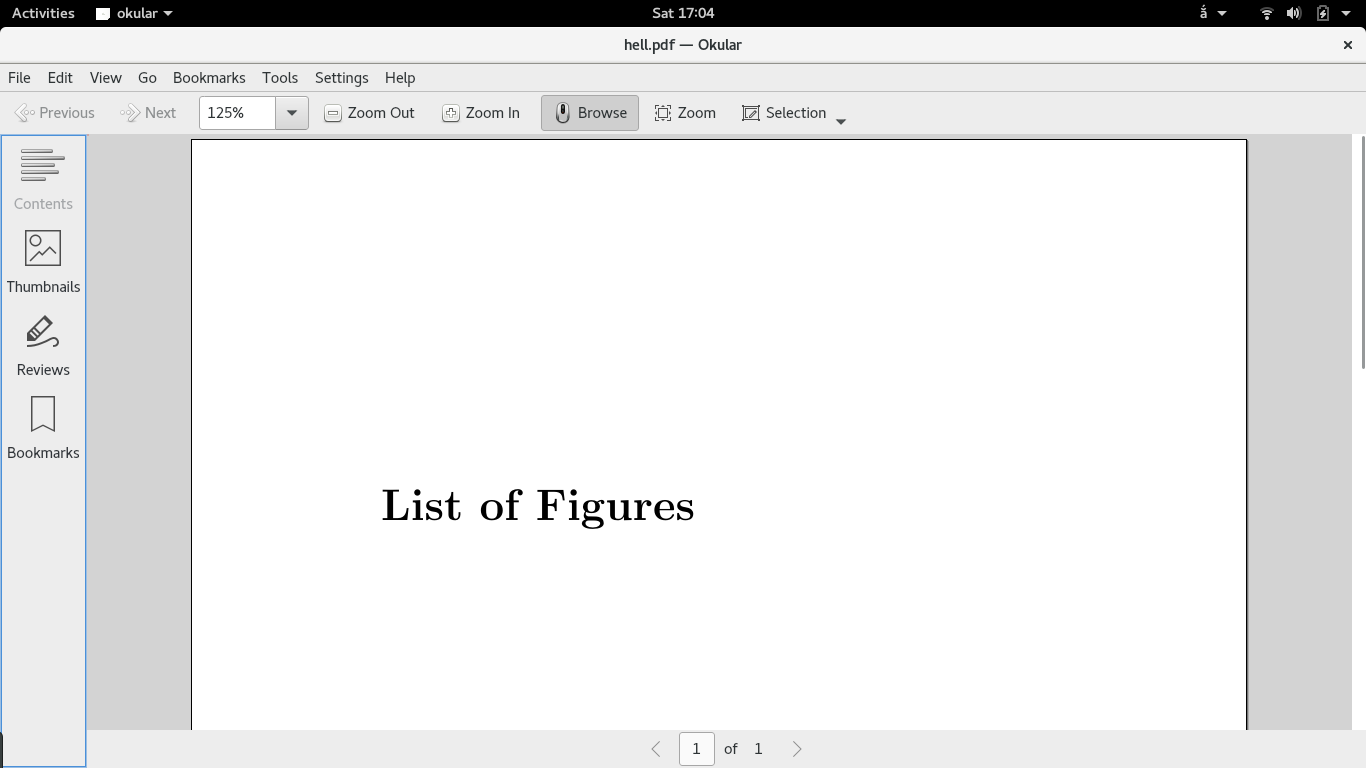
\includegraphics[width=1.\linewidth]{tocloft_a}
  \caption{Sử dụng class \texttt{book}}
  \label{fig:tocloft_a}
 \end{subfigure}
 \begin{subfigure}{0.5\textwidth}
  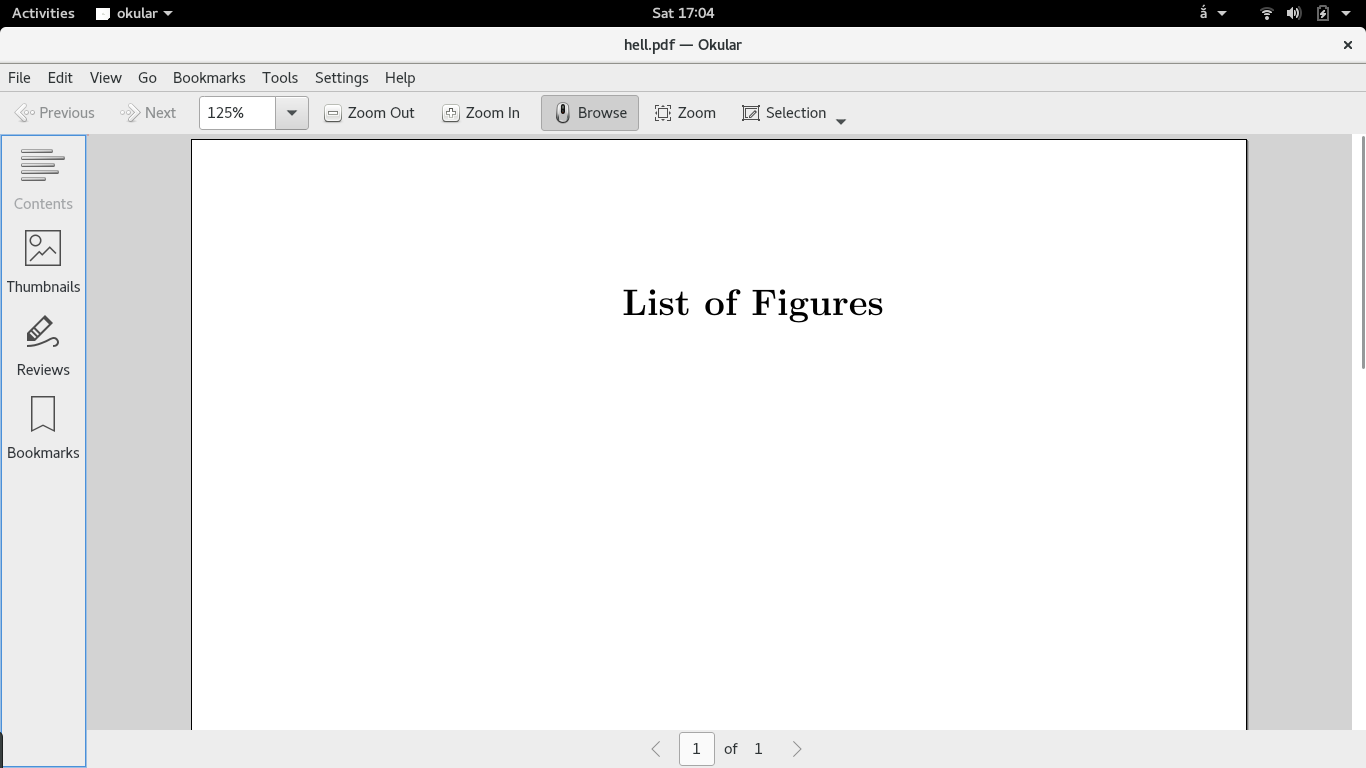
\includegraphics[width=1.\linewidth]{tocloft_b}
  \caption{Sử dụng class \texttt{vlththesis}}
  \label{fig:tocloft_b}
 \end{subfigure}

 \caption{So sánh tiêu đề danh sách hình vẽ của hai class văn bản}
 \label{fig:tocloft}
\end{figure}

Điều tương tự cũng xảy ra khi sử dụng \path|\listoftables| và \path|\tableofcontents|:\par

\begin{figure}[H] 
 \begin{subfigure}{0.5\textwidth}
  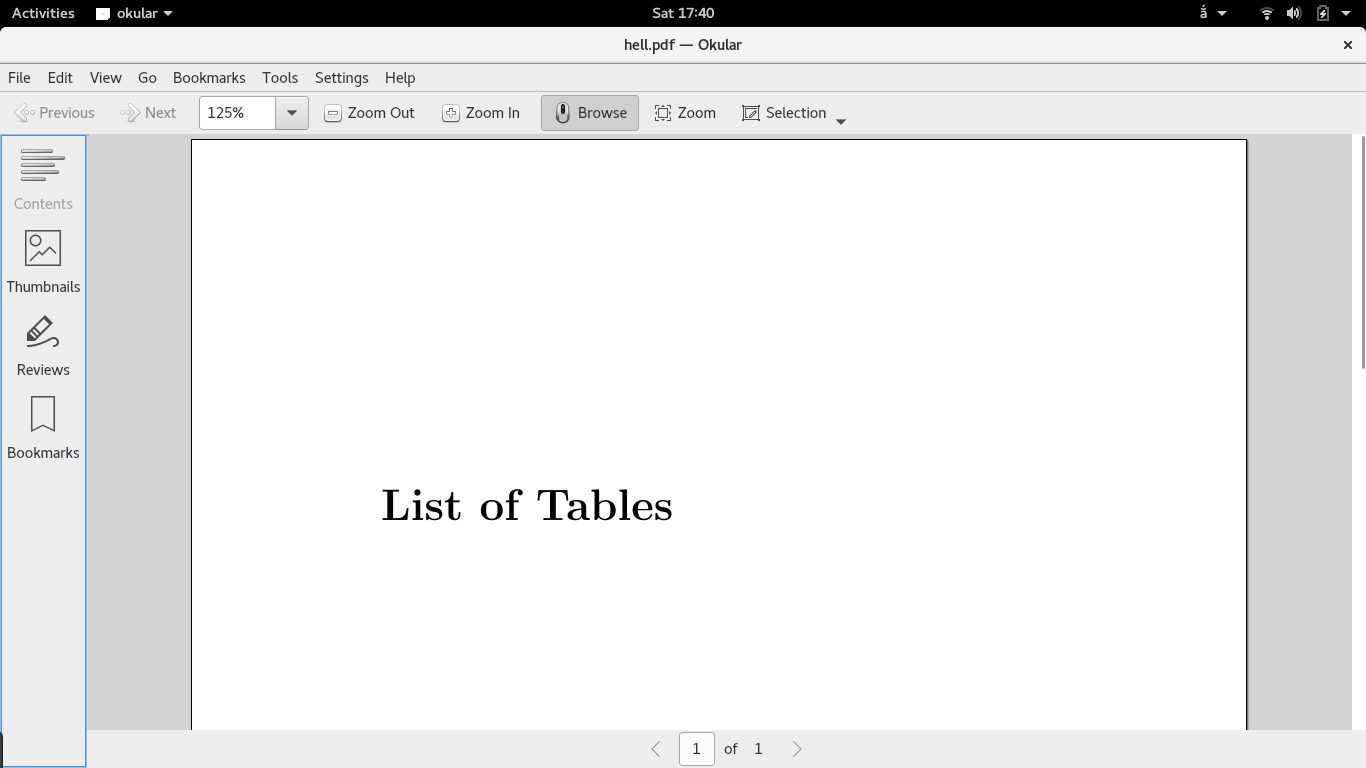
\includegraphics[width=1.\linewidth]{tocloft1_a}
  \caption{Sử dụng class \texttt{book}}
  \label{fig:tocloft1_a}
 \end{subfigure}
 \begin{subfigure}{0.5\textwidth}
  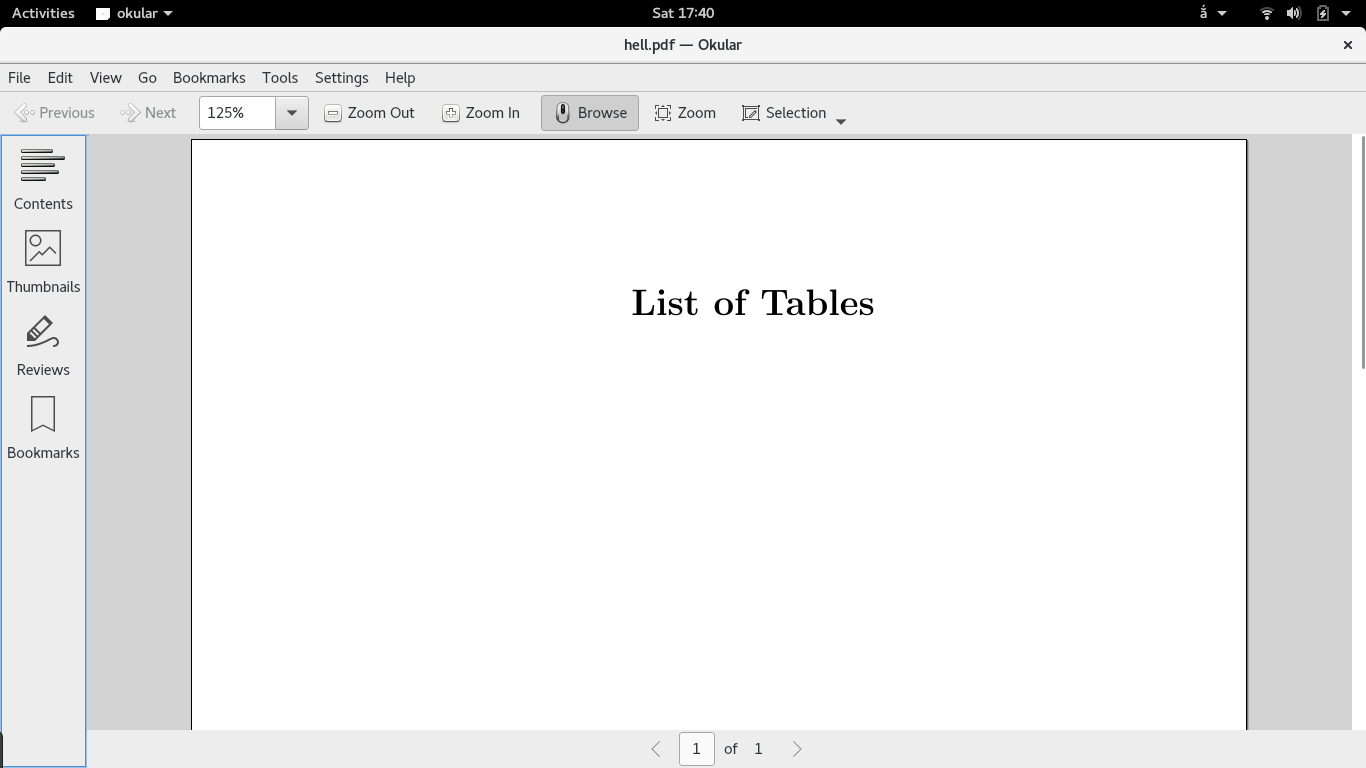
\includegraphics[width=1.\linewidth]{tocloft1_b}
  \caption{Sử dụng class \texttt{vlththesis}}
  \label{fig:tocloft1_b}
 \end{subfigure}

 \begin{subfigure}{0.5\textwidth}
  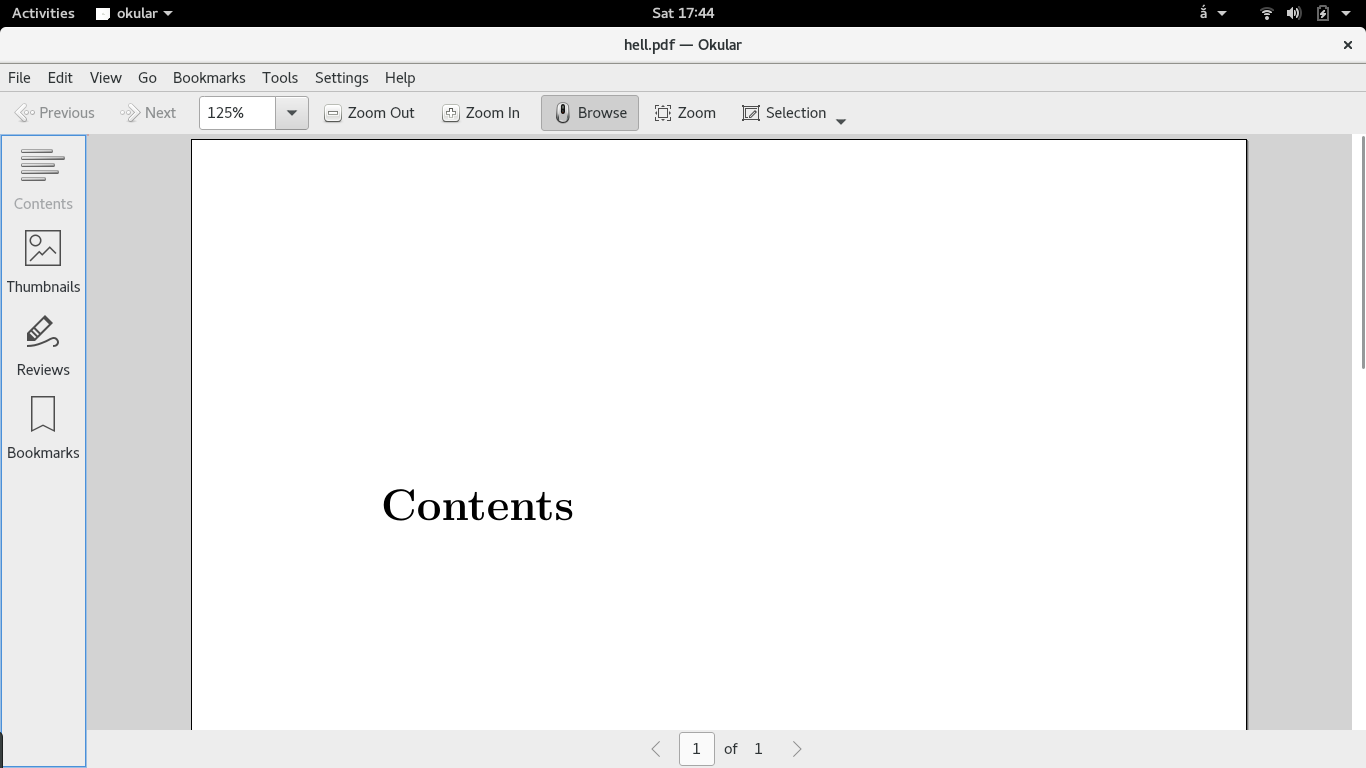
\includegraphics[width=1.\linewidth]{tocloft2_a}
  \caption{Sử dụng class \texttt{book}}
  \label{fig:tocloft2_a}
 \end{subfigure}
 \begin{subfigure}{0.5\textwidth}
  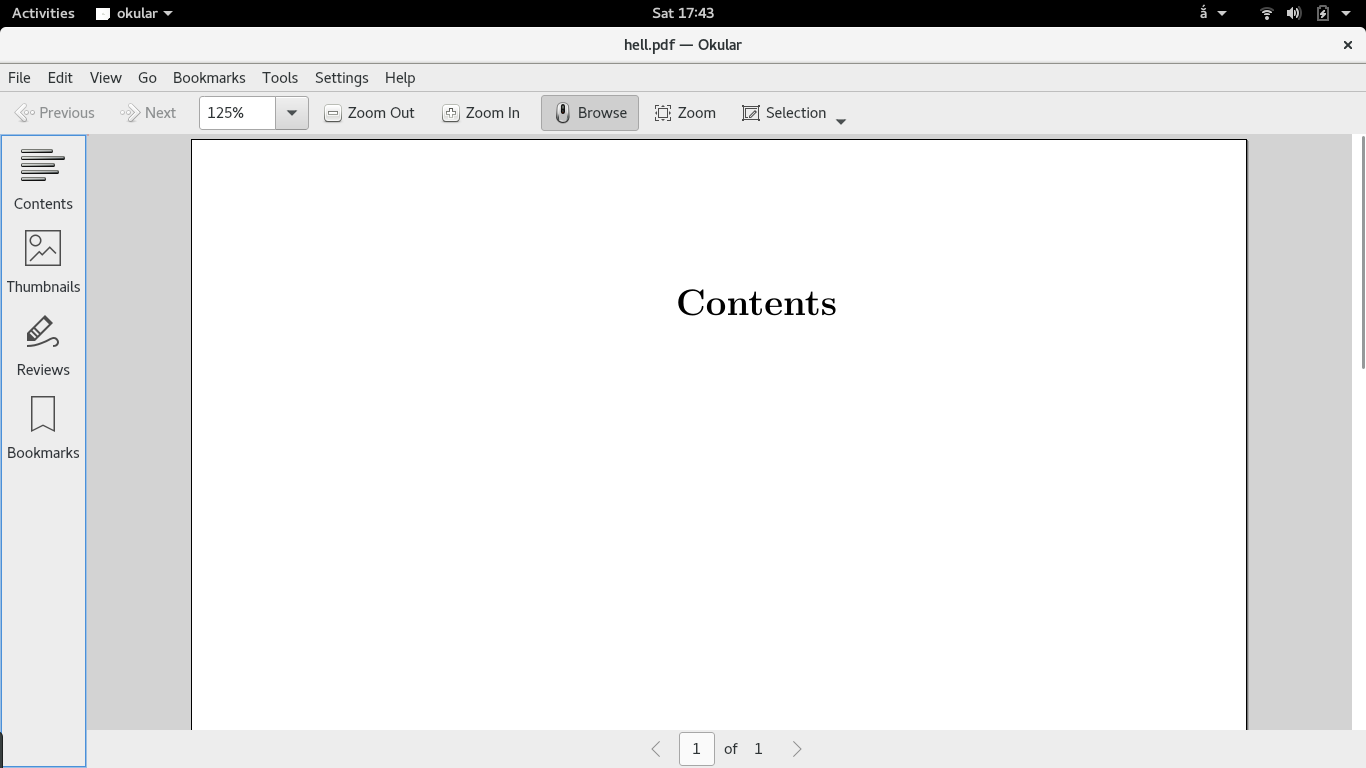
\includegraphics[width=1.\linewidth]{tocloft2_b}
  \caption{Sử dụng class \texttt{vlththesis}}
  \label{fig:tocloft2_b}
 \end{subfigure}
 
 \caption{So sánh tiêu đề danh sách bảng và mục lục của hai class văn bản}
 \label{fig:tocloft1}
\end{figure}
\clearpage
Tiếp theo là định dạng dành cho thành phần trong danh sách hình và bảng.\par
\lstinputlisting[firstline=168,lastline=175,firstnumber=168]{vlththesis.cls}

Trước hết ta xét cách trình bày mặc định các thành phần trong danh sách hình vẽ và bảng nếu không có các câu lệnh trên:\par
\begin{figure}[H] 
 \begin{subfigure}{0.5\textwidth}
  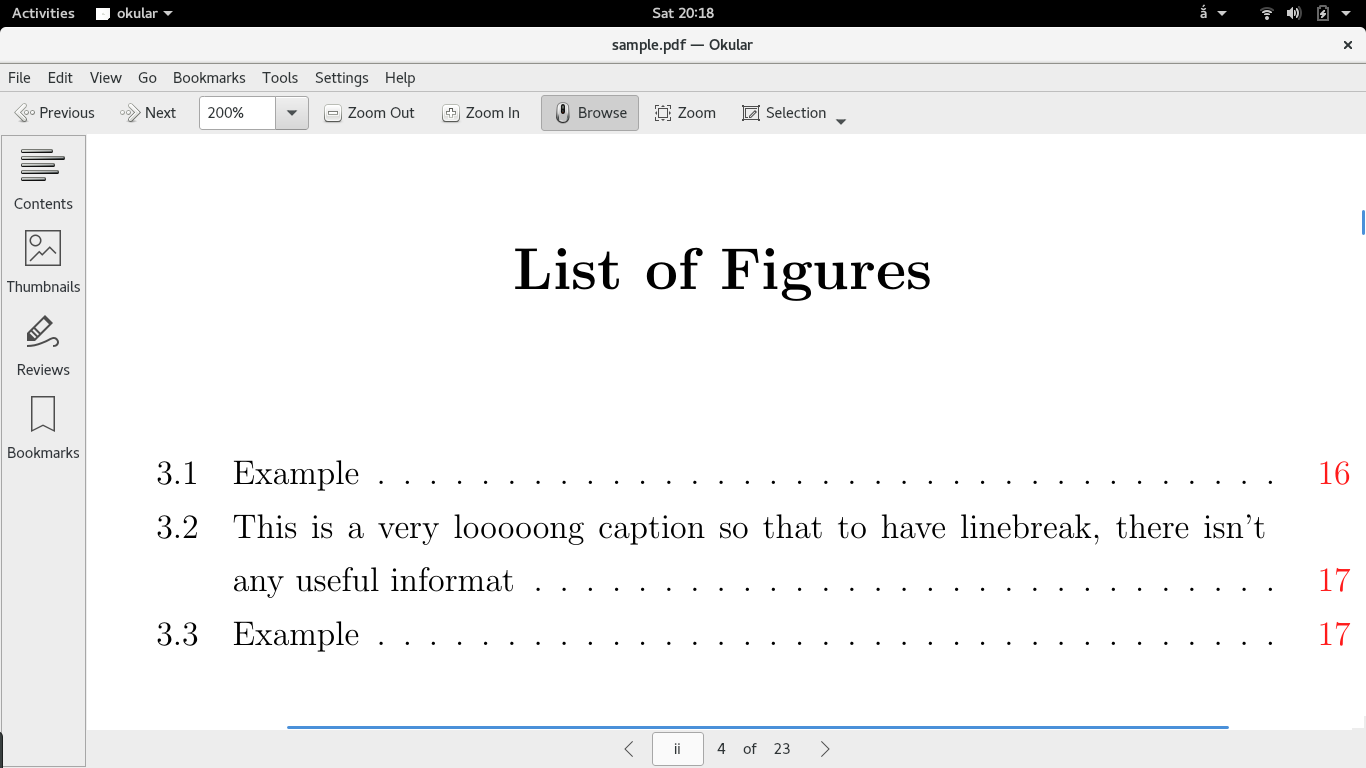
\includegraphics[width=1.\linewidth]{lof}
  \caption{Danh sách hình vẽ}
  \label{fig:lof}
 \end{subfigure}
 \begin{subfigure}{0.5\textwidth}
  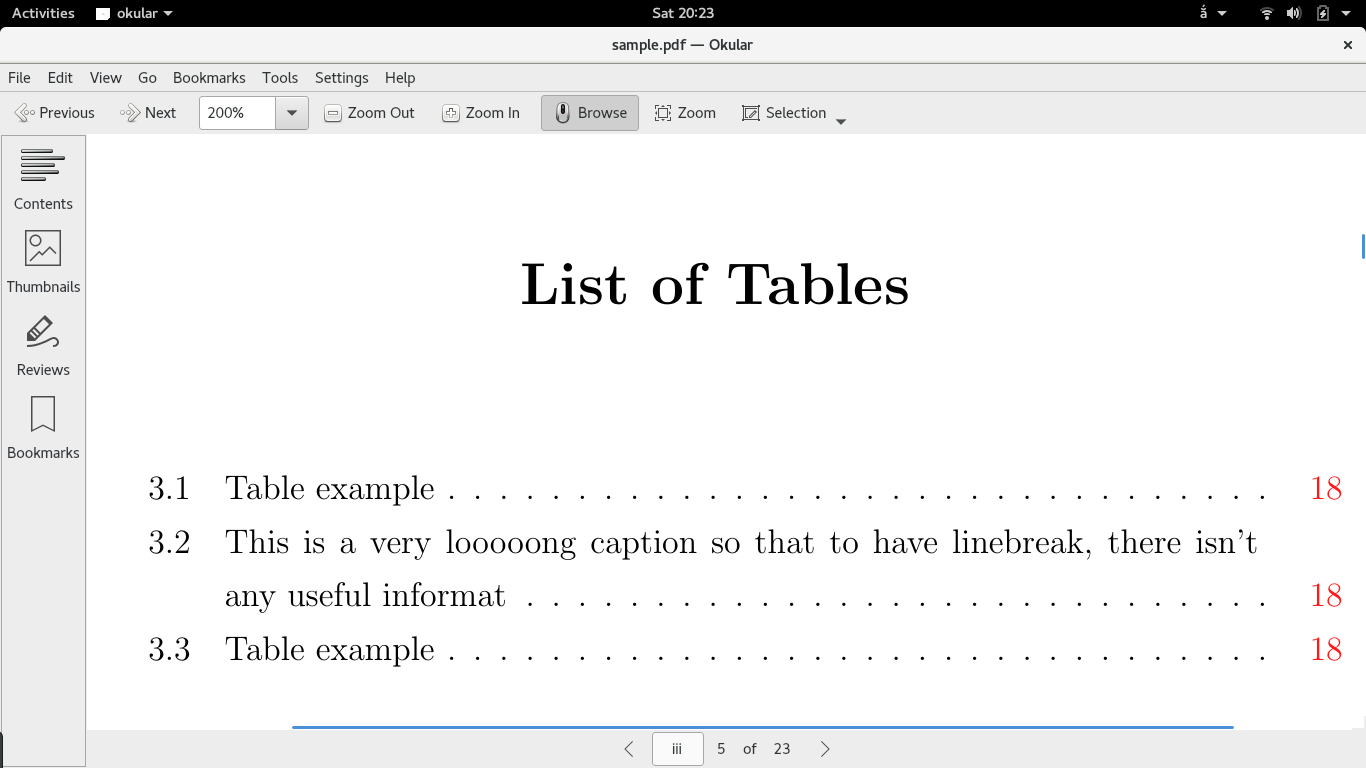
\includegraphics[width=1.\linewidth]{lot}
  \caption{Danh sách bảng}
  \label{fig:lot}
 \end{subfigure}

 \caption{Định dạng mặc định của LaTeX dành cho thành phần danh sách}
 \label{fig:loft}
\end{figure}

Như ta có thể thấy, các hình chỉ có nhãn là số hiệu, để thêm chữ “Hình”, “Bảng” (hoặc “Figure”, “Table”,\dots tuỳ theo ngôn ngữ khai báo 
trong \texttt{babel}), các giá trị đó, nếu có, sẽ được lưu trong macro \path|\cftZpresnum| của \texttt{tocloft} (Z là fig hoặc tab tương ứng với hình và bảng).
Bên cạnh đó, \path|\figurename|, \path|\tablename| là hai macro hệ thống LaTeX dùng để lưu giữ nhãn của hình và bảng bằng nhiều ngôn ngữ khác nhau (được sử
dụng làm nhãn cho caption). Do đó,
bằng cách sử dụng câu lệnh \path|\renewcommand|, ta có thể dùng macro của LaTeX để định nghĩa \path|\cftZpresnum| vốn đang bị trống theo
mặc định. Sau khi bổ sung nhãn đó ta lại xuất hiện hiện tượng nhãn và caption bị chồng lên nhau.\par
\begin{figure}[H] 
 \begin{subfigure}{0.5\textwidth}
  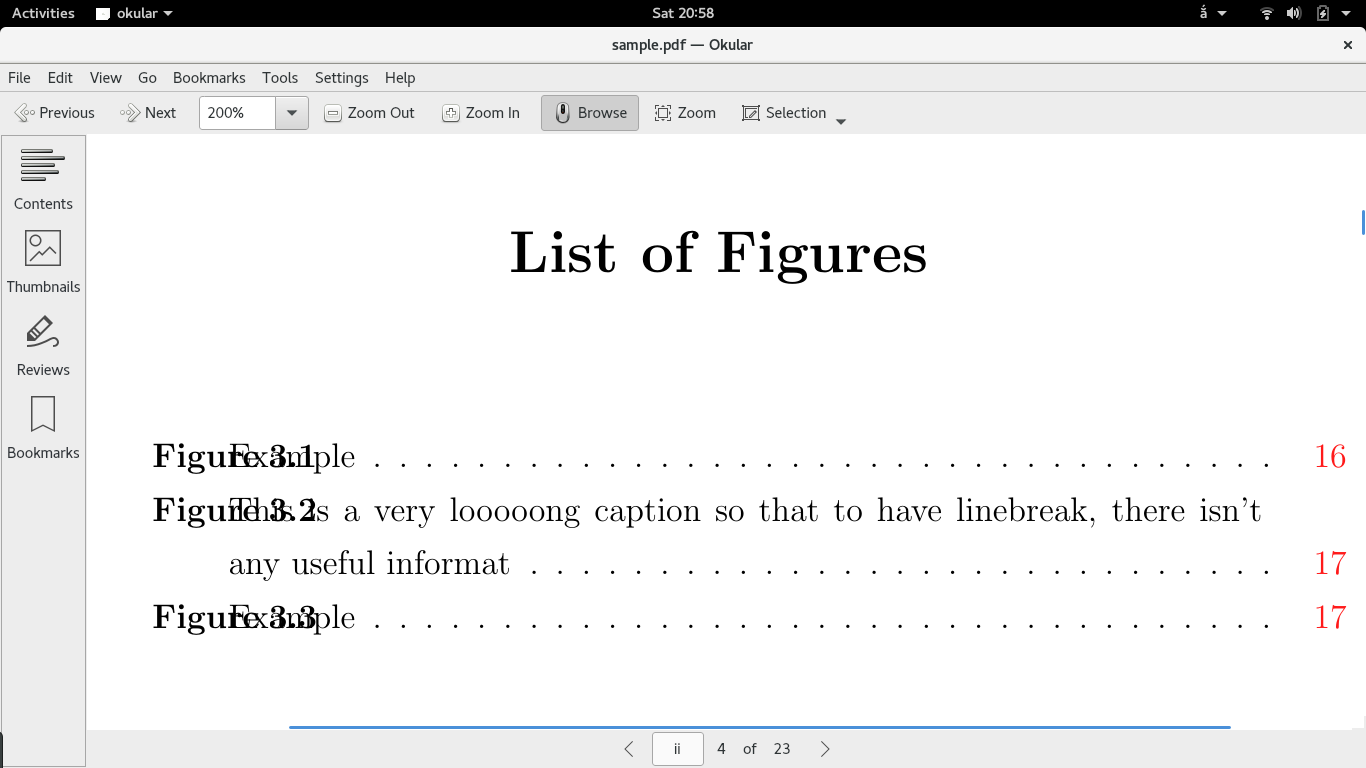
\includegraphics[width=1.\linewidth]{lof_er}
  \caption{Danh sách hình vẽ}
  \label{fig:lof_er}
 \end{subfigure}
 \begin{subfigure}{0.5\textwidth}
  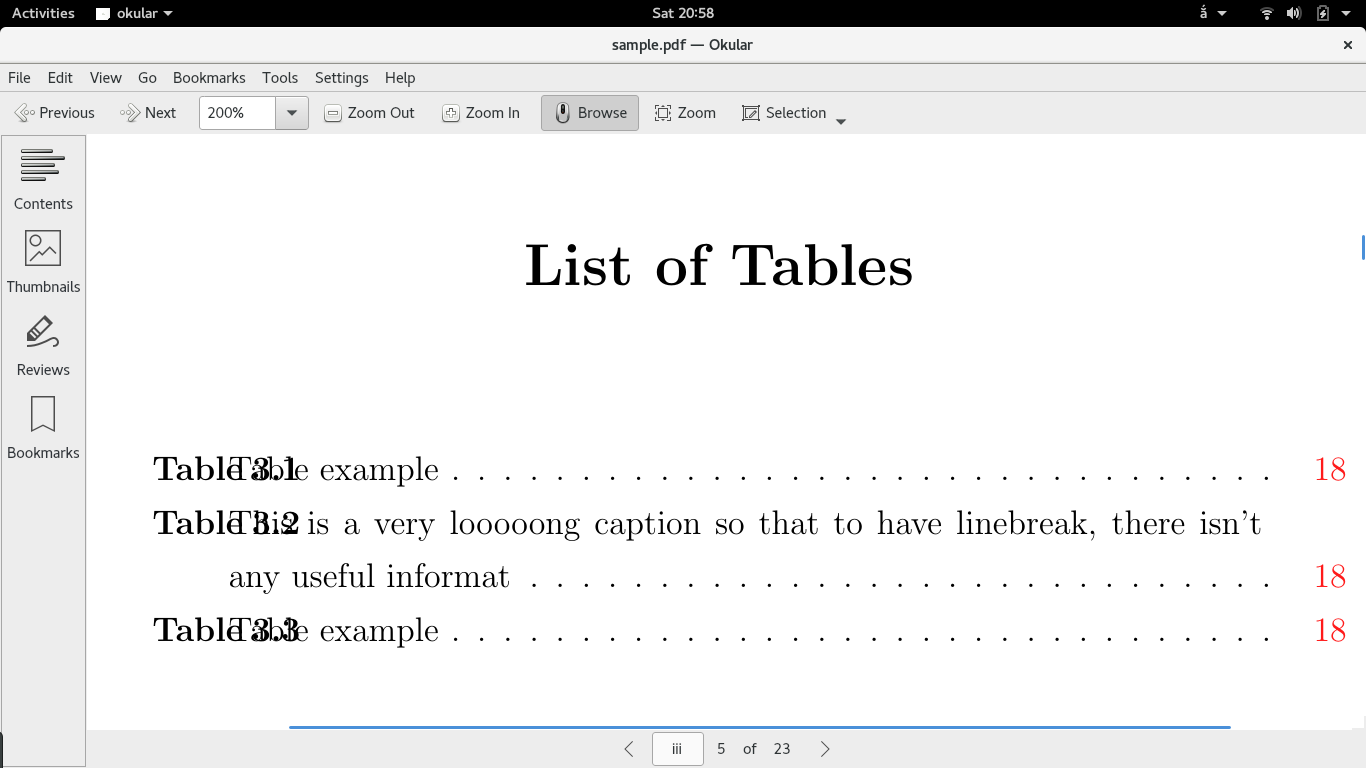
\includegraphics[width=1.\linewidth]{lot_er}
  \caption{Danh sách bảng}
  \label{fig:lot_er}
 \end{subfigure}

 \caption{Nội dung và nhãn bị chồng nhau sau câu lệnh bổ sung}
 \label{fig:loft_er}
\end{figure}

Để khắc phục điều này, ta cần thay đổi khoảng cách giữa nhãn và tiêu đề, được lưu trong macro \path|\cftZnumwidth|, bằng cách
tăng khoảng cách cũ bằng đúng với chiều dài của nhãn. Điều đó được thực hiện bằng các câu lệnh ở dòng 169-171 và 174-175. Sau
khi triển khai các câu lệnh đó ta được như sau.\par
\begin{figure}[H] 
 \begin{subfigure}{0.5\textwidth}
  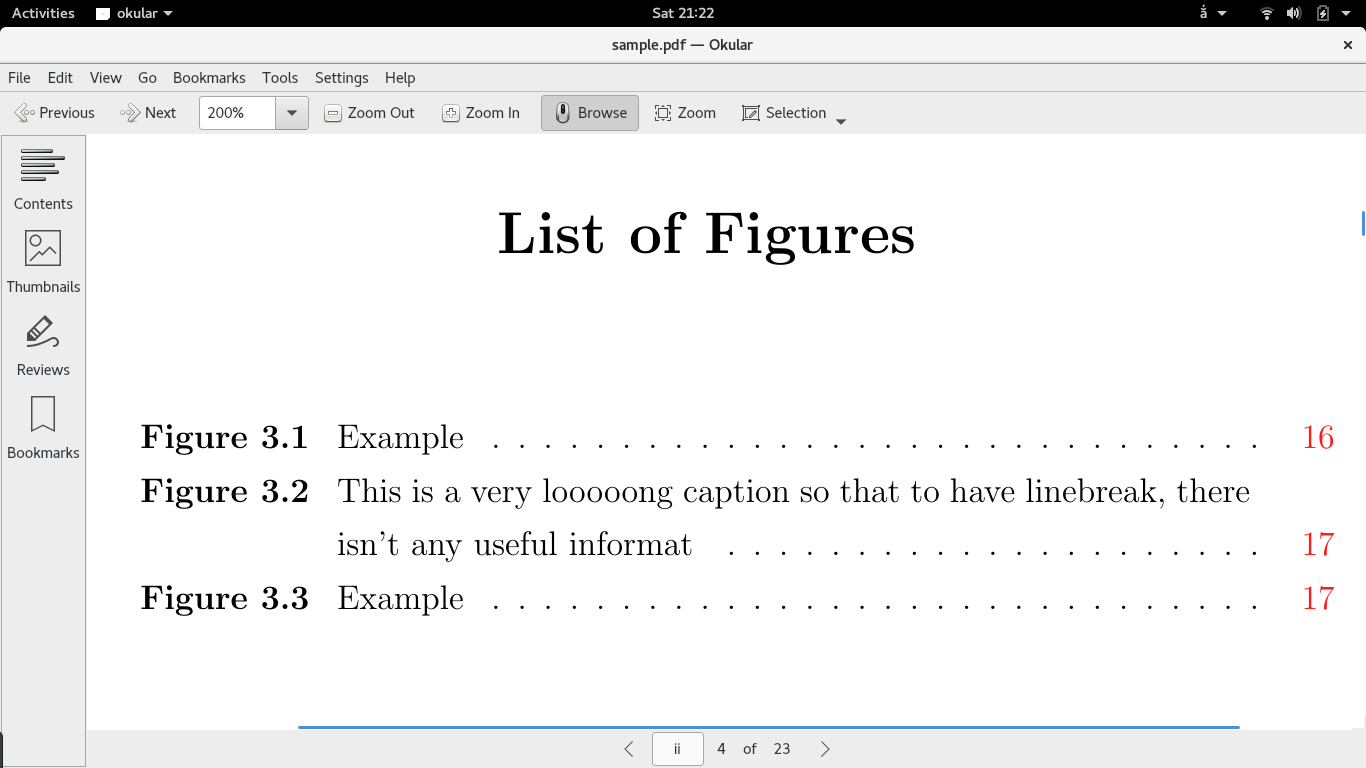
\includegraphics[width=1.\linewidth]{lof_new}
  \caption{Danh sách hình vẽ}
  \label{fig:lof_new}
 \end{subfigure}
 \begin{subfigure}{0.5\textwidth}
  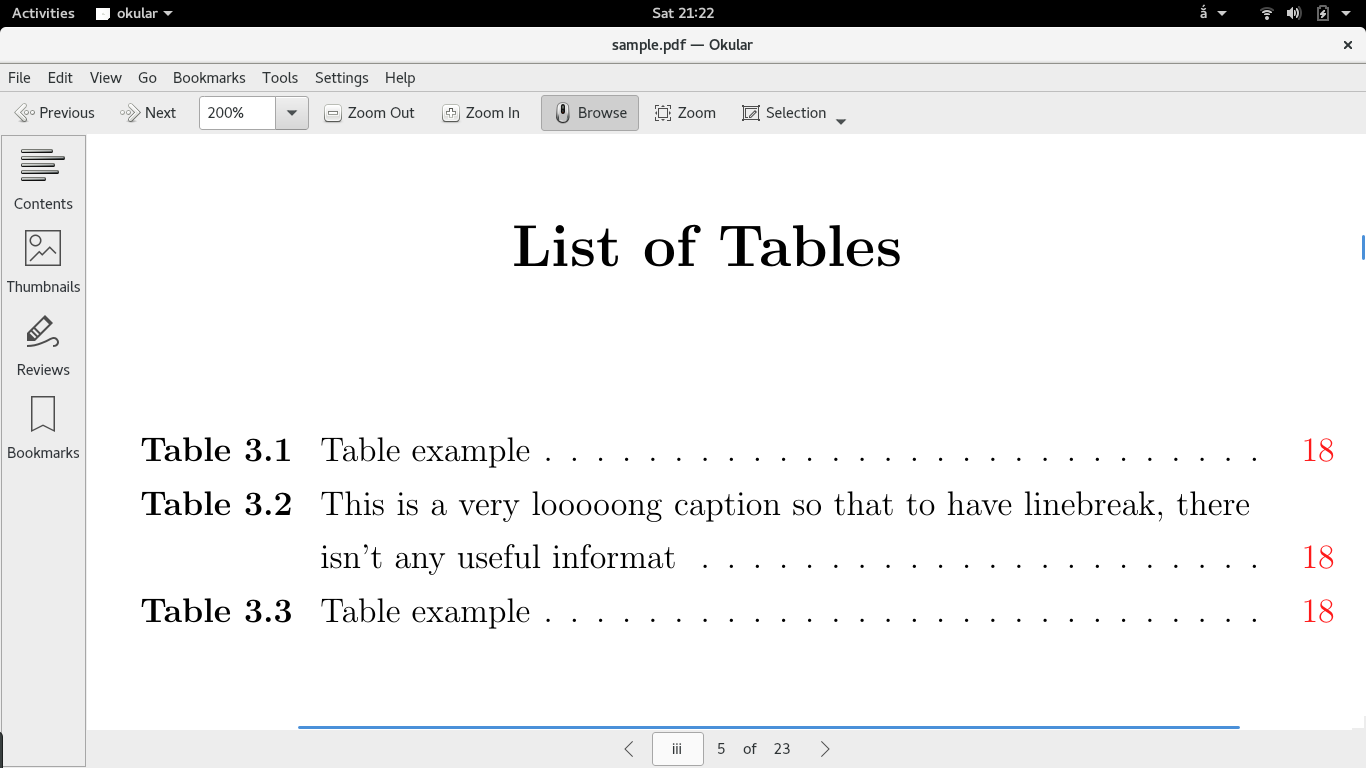
\includegraphics[width=1.\linewidth]{lot_new}
  \caption{Danh sách bảng}
  \label{fig:lot_new}
 \end{subfigure}

 \caption{Kết quả mong muốn của class}
 \label{fig:loft_new}
\end{figure}

Khai báo tiếp theo là cho package tạo danh sách kí hiệu viết tắt.\par
\lstinputlisting[firstline=177,lastline=177,firstnumber=177]{vlththesis.cls}

Package này cung cấp các câu lệnh giúp ta định nghĩa chữ viết tắt, các thuật ngữ, sử dụng option \textbf{acronym} cho phép
ta tiếp cận các câu lệnh dành cho việc định nghĩa, tạo liên kết, sắp xếp, xây dựng và in danh sách các kí hiệu viết tắt.
Để tạo danh sách này, ở phần tiền tố, người dùng sử dụng câu lệnh \path|\makenoidxglossaries| (\emph{không} phải là \path|\makeglossaries|,
tham khảo tài liệu \cite{glossaries} để biết thêm chi tiết), sau đó dùng câu lệnh \path|\newacronym{nhãn}{chữ viết tắt}{nghĩa đầy đủ}|
để định nghĩa chữ viết tắt như ví dụ sau:\par
\begin{verbatim}
\makenoidxglossaries

\newacronym{gcd}{GCD}{Greatest Common Divisor}
 
\newacronym{lcm}{LCM}{Least Common Multiple}
\end{verbatim}

Sau khi đã định nghĩa, người dùng được cung cấp ba câu lệnh \path|\acrshort{nhãn}, \acrlong{nhãn}| và \path|\acrfull{nhãn}| để
trình bày chữ viết tắt đã định nghĩa như sau:\par
\begin{verbatim}
\acrshort{lcm} is also called \acrlong{lcm}, as opposed to \acrfull{gcd}
\end{verbatim}
\begin{figure}[H]
 \centering
 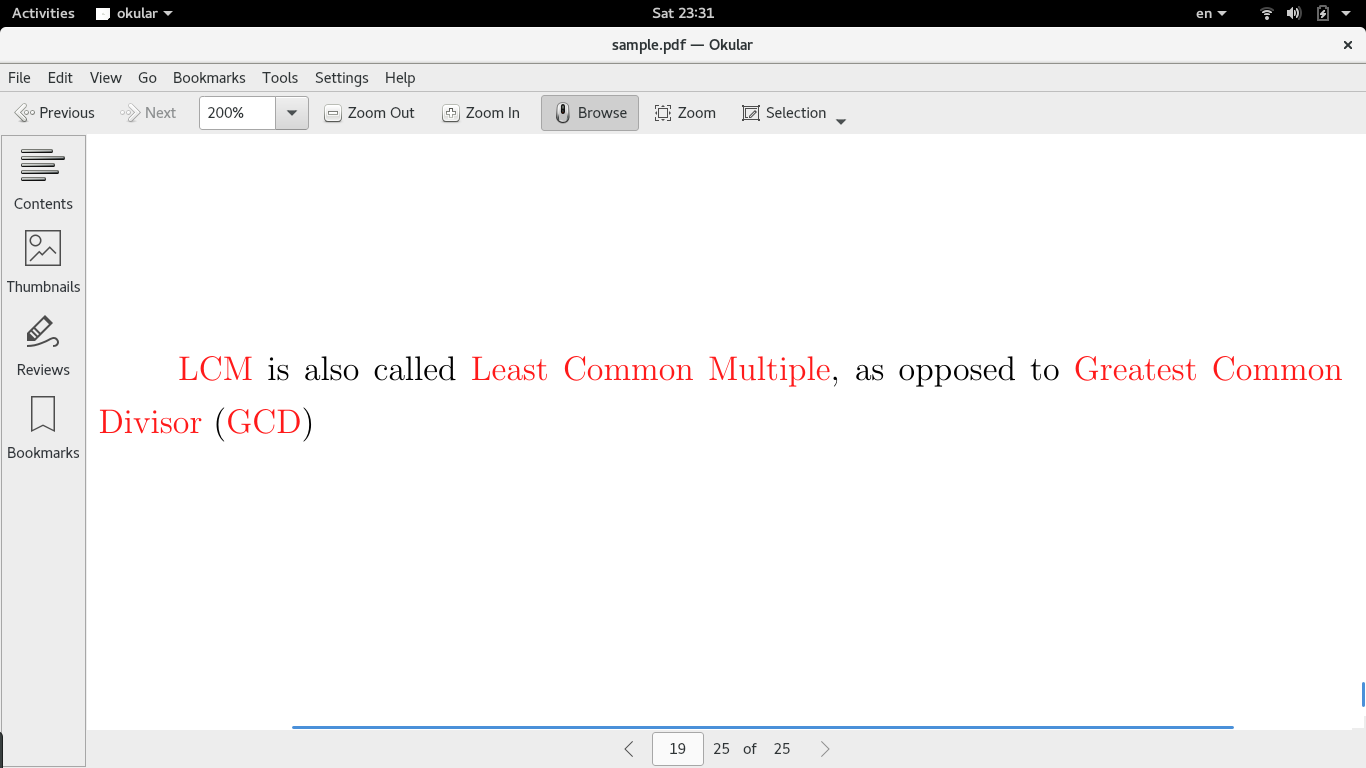
\includegraphics[width=0.7\textwidth]{acrexemple}
 \caption{Ví dụ package \texttt{glossaries}}
 \label{fig:acr}
\end{figure}

Để in danh sách, ta sử dụng \path|\printnoidxglossary[type=\acronymtype]| ở vị trí muốn in danh sách các từ viết tắt, người dùng
muốn biết thêm các câu lệnh và option cho \path|\printnoidxglossary| có thể tham khảo tài liệu hướng dẫn \cite{glossaries}. Lưu ý rằng
LaTeX chỉ in những chữ được tham chiếu trong văn bản \emph{ít nhất một lần}.\par
Tiếp theo là ba câu lệnh canh chỉnh cho đoạn văn (paragraph).\par
\lstinputlisting[firstline=179,lastline=181,firstnumber=179]{vlththesis.cls}

Câu lệnh \path|\setlength| dùng để định giá trị cho các macro quy định khoảng cách trong đó: \path|\parkip| là khoảng cách giữa các
đoạn văn, \path|\parindent| là khoảng cách thụt đầu dòng của dòng đầu tiên của các đoạn văn. Câu lệnh \path|\linespread| dùng để
định khoảng cách giữa các dòng trong cùng một đoạn văn, với \path|\linespread{1.3}| tương đương \texttt{1.5 line} trong trình
soạn thảo Microsoft Word. Trong ba giá trị trên \path|\parindent| và \path|\linespread| dựa trên mẫu báo cáo khoá luận chuẩn của bộ
môn.\par 

\subsection{Các câu lệnh của class}\label{sec:3.3.3}
Ngoài tích hợp sẵn các package đưa ra các thiết lập mặc định, class cũng có các câu lệnh riêng.\par~\par


\textbullet\ {\large\path|\supervisorName{text}|}\par~\par
Câu lệnh này cho phép người dùng khai báo tên của cán bộ hướng dẫn (CBHD) ở phần tiền tố, câu lệnh này được định nghĩa như sau:

\lstinputlisting[firstline=221,lastline=222,firstnumber=221]{vlththesis.cls}

Câu lệnh này sẽ đẩy tên CBHD vào macro \path|\thesupervisorName| để sử dụng cho câu lệnh dưới đây.\par~\par

\textbullet\ {\large\path|\printcoverpage|}\par~\par

Câu lệnh này được định nghĩa sử dụng các macro đã được định nghĩa trước và các câu lệnh trong LaTeX để thiết kế bố cục cho trang
bìa của bài báo cáo theo đúng mẫu chuẩn của khoá luận. Người dùng cần sử dụng các câu lệnh khai báo của LaTeX là \path|\title{text}|,
\path|\author{text}| và câu lệnh \path|\supervisorName{text}| của class để cung cấp tiêu đề báo cáo (tên đề tài), tên người thực hiện
và CBHD cho câu lệnh sử dụng nhằm xây dựng trang bìa. Trường hợp có nhiều hơn một người thực hiện hay hướng dẫn, người dùng hãy trình
bày theo ví dụ sau để đảm bảo class trình bày đúng bố cục: \path|\author{Nguyen Thi A\\  &Tran Thi B \\ &Vo Van C}|. 
Người dùng cũng thực hiện tương tự với câu lệnh \path|\supervisorName{text}|. Trang bìa của báo cáo này được in ra
sử dụng chính câu lệnh trên. Định nghĩa chi tiết của câu lệnh được nêu ở phần phụ lục \ref{append:A}.\par 
Ý tưởng câu lệnh này dựa trên câu lệnh tương tự của class \texttt{gsemthesis} \cite{gsem}.\par
\clearpage

\textbullet\ {\large\path|\acknowledgements{text}|}\par~\par

Câu lệnh này dùng để đẩy “Lời cảm ơn” vào macro \path|\theacknowledgements|, người dùng có thể soạn trực tiếp lời cảm ơn vào
giữa \textsl{text} của câu lệnh, hoặc soạn riêng một file \texttt{.tex} (file này không cần thiết phải có các câu lệnh LaTeX)
cho lời cảm ơn và sử dụng lệnh \path|\input{file}| để trỏ file đó vào câu lệnh (\path|\acknowledgements{\input{file}}|).\par~\par

\textbullet\ {\large\path|\printfrontmatter|}\par~\par

Đây là câu lệnh dùng để in Lời cảm ơn, Mục lục, Các kí hiệu viết tắt, Danh sách hình vẽ, Danh sách bảng theo đúng thứ tự liệt kê như
trên. Đối với Lời cảm ơn, \path|\printfrontmatter| sử dụng macro \path|\theacknowledgements|, câu lệnh ẩn số trang \\ (\path|\pagenumbering{gobble}|), sử dụng \path|\chapter*|
để đặt tiêu đề Lời cảm ơn,\dots Tiếp theo, câu lệnh tích hợp \path|\tableofcontents| nhằm in ra Mục lục, để in Danh sách hình vẽ và
Danh sách bảng, câu lệnh \path|\printfrontmatter| sau đó sử dụng \path|\conditionalLoF| và  \path|\conditionalLoT|, hai biến thể của 
\path|\listoffigures| và \path|\listoftables| được định nghĩa trong class này như sau:\par
\lstinputlisting[firstline=293,lastline=294,firstnumber=293]{vlththesis.cls}

Sử dụng hai câu điều kiện \path|\iftotalfigures...\fi| và \path|\iftotaltables...\fi| của package \texttt{totalcount},
class kiểm tra xem người dùng có chèn hình và bảng vào văn bản (chỉ tính những hình sử dụng môi trường \textbf{\slshape figure} và bảng sử
dụng môi trường \textbf{\slshape table} chứa \textbf{\slshape tabular}) trước khi quyết định in danh sách.\par

Câu lệnh sử dụng \path|\printnoidxglossary[type=\acronymtype,title=\acrtitle, style=listdotted]| để in Các kí hiệu viết tắt, và được 
kiểm tra bởi câu điều kiện \path|\iftoggle{noacr}|, class cung cấp option \textbf{noarc} để người dùng sử dụng trong trường hợp
không muốn in danh sách chữ viết tắt hay hoàn toàn không sử dụng chữ viết tắt nào trong văn bản, khi đó người dùng cần khai báo
option này để ngăn không cho class in danh sách. Key \texttt{title} của câu lệnh \path|\printnoidxglossary| được truyền vào value là
một macro \path|\acrtitle| với định nghĩa như sau:\par
\clearpage 
\begin{lstlisting}[firstnumber=287,escapeinside={(*}{*)}]
\iftoggle{viet}{%
	\def\acrtitle{(*Các kí hiệu viết tắt*)}%
}{%
	\def\acrtitle{Acronym}%
}
\end{lstlisting}

Câu điều kiện \path|\iftoggle{viet}| kiểm tra option \textbf{vietnamese} của class nhằm định nghĩa giá trị thích hợp cho macro. Thêm
vào đó câu lệnh tích hợp câu \path|\frontmatter| và \path|\mainmatter| của class \texttt{book} để đánh số trang la mã
cho các đối tượng trên và trả về số thường cho các chương chính. Định nghĩa đầy đủ của câu lệnh này được liệt kê trong phụ lục \ref{append:A}. 
Lời cảm ơn, Mục lục, Các kí hiệu viết tắt, Danh sách hình, bảng của báo cáo này được tổng hợp và in ra tự động sử dụng duy nhất 
một câu lệnh này.\par~\par

\textbullet\ {\large\path|\startintroduction|}\par~\par

Đây là câu lệnh dùng để thay thế cho \path|\chapter*{Lời giới thiệu}| hay \path|\chapter*{Introduction}|, định nghĩa của câu lệnh này như
sau:\par
\begin{lstlisting}[firstnumber=338,escapeinside={(*}{*)}]
\newcommand{\startintroduction}{%
		\iftoggle{viet}{
		\chapter*{(*Lời giới thiệu*)}
		\markboth{}{(*Lời giới thiệu*)}
		\addcontentsline{toc}{chapter}{(*Lời giới thiệu*)}%
		}{%
		\chapter*{Introduction}
		\markboth{}{Introduction}
		\addcontentsline{toc}{chapter}{Introduction}%
		}\label{ch:intro}
}
}
\end{lstlisting}

Ta có thể thấy, câu lệnh này kèm theo \path|\iftoggle{viet}| để kiểm tra option của class nhằm đưa giá trị thích hợp làm tiêu đề.
Câu \path|\addcontentsline| để đưa Lời giới thiệu vào mục lục (mặc định LaTeX không đưa các chương không đánh số vào mục lục)
và \path|\markboth| để cập nhật lại header.\par

Hai câu lệnh \path|\printfrontmatter| và \path|\startintroduction| trên cũng lấy ý tưởng từ hai câu lệnh cùng tên của class 
\texttt{gsemthesis} \cite{gsem}.\par


\textbullet\ {\large\path|\thebackmatter|}\par~\par

Câu lệnh này dùng để đánh dấu bắt đầu phụ lục, tất cả các \path|\chapter| sau câu lệnh này đề được hiểu và sẽ được LaTeX dán nhãn phụ
lục và đánh số bằng chữ cái, ví dụ “Phụ lục A”, “Phụ lục B”,\dots Định nghĩa của câu lệnh này như sau:\par
\lstinputlisting[firstline=351,lastline=357,firstnumber=351]{vlththesis.cls}

Hai câu lệnh \path|\titleformat| và \path|\titlespacing*| dùng để tinh chỉnh lại đề mục cho phụ lục, loại bỏ các đường kẻ và dời lên
đầu trang một khoảng ngắn, phụ lục của báo cáo này là kết quả, đồng thời, câu lệnh định lại style cho các trang sau câu lệnh thành
\texttt{supplement} (được đề cập ở \hyperlink{appendix}{3.3.2} dòng lệnh 101-106).\par~\par

\textbullet\ {\large\path|\reference|}\par~\par

Câu lệnh này dùng để thay thế cho \path|\printbibliography| kèm theo các biến đổi sau:\par
\lstinputlisting[firstline=359,lastline=363,firstnumber=359]{vlththesis.cls}

Câu \path|\backmatter| dùng để báo tất cả các câu lệnh chương mục sau câu lệnh này sẽ không được đánh số, đây chỉ là câu lệnh
đánh dấu các phần phụ trợ sau phần chính của sách, đồng thời định style \texttt{plain} cho Tài liệu tham khảo.\par

